\documentclass[12pt, a4paper, oneside]{book}
\usepackage[portuges]{babel}
\usepackage{amsmath,amssymb,amsxtra,latexsym}
\bibliographystyle{plain}
\usepackage[utf8]{inputenc}
\usepackage[T1]{fontenc}
\usepackage{graphicx}
\usepackage{listings}
\usepackage{courier}
\usepackage{graphics}
\usepackage{color} 
\usepackage{subcaption}
\usepackage{xspace}
\usepackage{mathtools}
\DeclarePairedDelimiter{\ceil}{\lceil}{\rceil}
\DeclarePairedDelimiter{\floor}{\lfloor}{\rfloor}

% ---------------------
% Definição das Margens
% ---------------------
\setlength{\textwidth}{16.0cm} %
\setlength{\textheight}{23.5cm} %
\setlength{\baselineskip}{0.6cm} %
\renewcommand{\baselinestretch}{1.1} %
%\setlength{\evensidemargin}{0.5cm} %
\setlength{\oddsidemargin}{0.00in} %
\setlength{\topmargin}{-1.0in} %
\setlength{\headsep}{0.5in} %
\setlength{\headheight}{0.2in} %

\setlength{\parindent}{0.0cm} %

% ---------------------
% Definição da listagem de código-fonte
% ---------------------
\lstset{
         basicstyle=\footnotesize\ttfamily, % Standardschrift
         %numbers=left,               % Ort der Zeilennummern
         numberstyle=\tiny,          % Stil der Zeilennummern
         %stepnumber=2,               % Abstand zwischen den Zeilennummern
         numbersep=5pt,              % Abstand der Nummern zum Text
         tabsize=2,                  % Groesse von Tabs
         extendedchars=true,         %
         breaklines=true,            % Zeilen werden Umgebrochen
         keywordstyle=\color{red},
    		frame=b,         
 %        keywordstyle=[1]\textbf,    % Stil der Keywords
 %        keywordstyle=[2]\textbf,    %
 %        keywordstyle=[3]\textbf,    %
 %        keywordstyle=[4]\textbf,   \sqrt{\sqrt{}} %
         stringstyle=\color{white}\ttfamily, % Farbe der String
         showspaces=false,           % Leerzeichen anzeigen ?
         showtabs=false,             % Tabs anzeigen ?
         xleftmargin=17pt,
         framexleftmargin=17pt,
         framexrightmargin=5pt,
         framexbottommargin=4pt,
         %backgroundcolor=\color{lightgray},
         showstringspaces=false      % Leerzeichen in Strings anzeigen ?        
 }
 \lstloadlanguages{
         C++
 }

 \usepackage{caption}
\DeclareCaptionFont{white}{\color{white}}
\DeclareCaptionFormat{listing}{\colorbox[cmyk]{0.43, 0.35, 0.35,0.01}{\parbox{\textwidth}{\hspace{15pt}#1#2#3}}}
\captionsetup[lstlisting]{format=listing,labelfont=white,textfont=white, singlelinecheck=false, margin=0pt, font={bf,footnotesize}}

\renewcommand\lstlistingname{Código}
\renewcommand\lstlistlistingname{Códigos}
% FIM da definição da listagem de código-fonte
% ---------------------

\hyphenation{ge-ra-ção}

\setcounter{page}{1}

% configurações de conteúdo

\newcommand{\autor}{Rafael Cerqueira de Campos}

\newcommand{\titulo}{Implementação de Texturas 3D para Renderização de
Volumes no Blender}

\newcommand{\orientador}{Prof. Dr. Mario Augusto de Souza Liziér}

\newcommand{\coorientador}{}

% FIXME Substituir 'Ano' pelo ano em que ocorreu sua defesa.
\newcommand{\ano}{2013}


%% fim - configurações de conteúdo


\newcommand{\bit}{{\it bit}\xspace}
\newcommand{\bits}{{\it bits}\xspace}

\newcommand{\buffer}{{\it buffer}\xspace}
\newcommand{\buffers}{{\it buffers}\xspace}

\newcommand{\voxel}{\emph{voxel}\xspace}
\newcommand{\voxels}{\emph{voxels}\xspace}

\newcommand{\grid}{\emph{grid}\xspace}
\newcommand{\grids}{\emph{grids}\xspace}

%onde estão as imagens!
\graphicspath{{images/}}


\begin{document}

\frontmatter
%

\includegraphics[width=.94in, height=1in, keepaspectratio=true]{images/LogoUFSCar}
\vspace*{1cm}
\begin{center}
    
	    {\large \scshape \bfseries Universidade Federal de São Carlos \\

    \vspace{.5cm}

    Centro de Ciências Exatas e de Tecnologia \\

     \vspace{.5cm}

   Departamento de Computação}
\end{center}
\vspace{2cm}
\begin{center}
    {\Large \scshape \autor}
\end{center}
\vspace{2cm}
\begin{center}
    {\Large \scshape \bfseries \titulo}
\end{center}
\vspace{2cm}
{\bfseries
\noindent
Orientador:  \orientador
}
\vspace{.25cm}
\vfill
\begin{center}
    % O tamanho da fonte deve ser 12pt em negrito.
    % Deve-se utilizar caixa alta.
    {\scshape \bfseries São Carlos \\ \ano}
\end{center}
 

\tableofcontents

\chapter{Introdução}

Em computação gráfica, objetos tridimensionais são geralmente representados apenas por sua superfície, por meio de malhas poligonais ou retalhos \emph{NURBS}\footnote{\emph{Non-Uniform Rational B-Spline}, na sigla em inglês, é um modelo matemático usado para gerar e representar curvas e superfícies.}. Quando estes modelos de representação são utilizados, as propriedades visuais do objeto, como cor, rugosidade e reflexividade, são definidas apenas na superfície do modelo e usadas pelos \emph{shaders}\footnote{\emph{Shaders}, de modo bem simplista, são sub-programas executados, em geral, nos processadores gráficos para a geração de imagens. Uma discussão mais extensa é apresentada na Seção \ref{shaders}.}, que podem ser simples, como um modelo de reflexão difusa ou tão complexo quanto uma \emph{BRDF}\footnote{\emph{Bidirectional Reflectance Fistribution Function}, na sigla em inglês, é uma função de quatro dimensões que define como a luz é refletida em uma superfície opaca.}. O que ocorre nestes casos é o cálculo do transporte de luz estritamente nos pontos da superfície do modelo. Logo, estes métodos não são capazes de avaliar as interações de luz que ocorrem no interior do objeto. \\


Comparada à renderização\footnote{\emph{Rendering}, processo de síntese de imagem a partir de cenas virtuais. Sem tradução direta, será utilizada uma adapatação para o português. } de superfícies, a renderização de volumes descreve uma gama de técnicas para gerar imagens a partir de dados escalares tridimensionais. Essas técnicas foram motivadas originalmente pela área de visualização científica, em que dados volumétricos são obtidos por medições ou simulações numéricas. Exemplos comuns são dados médicos do interior do corpo humano obtidos por tomografia computadorizada ou resonância magnética. Outros exemplos são dados de dinâmica dos fluidos computacional, dados geológicos, superfícies implícitas, entre outros. \\


Com a evolução de técnicas eficientes de renderização, dados volumétricos estão se tornando mais relevantes para aplicações em jogos digitais. Estes modelos volumétricos são ideais para descrever objetos dispersos, como fluidos, gases, e fenômenos naturais, como nuvens, névoa, fumaça e fogo. \\

O desafio de renderizar volumes está principalmente na avaliação da interação entre a luz e e os elementos naturais, como as nuvens. A luz pode ser absorvida, espalhada, ou emitida por materiais gasosos, e que participam na propagação luminosa. Essa interação precisa ser avaliada em todas as posições do volume tridimensional preenchido com o gás, tornando a renderização volumétrica uma tarefa com um alto custo computacional. 

%\section{Definição do Problema}

Como discutido, dados volumétricos são essenciais para várias aplicações em computação gráfica, como na produção de efeitos visuais e imagens médicas, incluindo simulação de fluidos, modelagem com superfícies implícitas e a própria renderização de volumes. \\


Na maioria das aplicações, os dados volumétricos são representados por imagens (ou \emph{grids}) tridimensionais regulares e espacialmente uniformes, em parte porque tais representações são computacionalmente simples. \emph{Grids} serão especificados mais detalhadamente na Seção \ref{texturas3d}.
%, mas trata-se basicamente de uma estrutura de três dimensões composta por elementos de volume - um exemplo uniforme é um cubo de lado igual a $10$, composto por pequenos cubos de lado $1$. Neste exemplo, os pequenos cubos são os elementos de volume que compõem o grid, o cubo maior. 

\subsection*{Abordagem básica à renderização de volumes}
\label{approach}

O processo de renderização de volumes, tal como tratado neste trabalho, foi dividido nas seguintes etapas, brevemente descritas a seguir. \\

\begin{itemize}
\item \emph{Consulta aos dados}. Posições no espaço são escolhidas para serem amostradas no volume, isto é, os pontos escolhidos pela aplicação são buscados na estrutura que armazena o volume. 

\item \emph{Interpolação}. Os pontos escolhidos na etapa anterior normalmente são diferentes dos pontos existentes no volume. Assim, um campo 3D contínuo precisa ser reconstruído a partir da imagem discreto para que os valores nos pontos buscados possam ser obtidos. 

\item \emph{Shading e Iluminação}. O modelo óptico do problema é calculado, e as componentes de absorção e emissão de luz são avaliados. Com os resultados da interação da luz com o volume, a imagem pode ser gerada.
\end{itemize}

As duas primeiras etapas, de consulta ao volume e cálculos de interpolação são processos estritamente locais em relação aos pontos amostrados. Dessa forma, em um software modular, é de se esperar que as implementações destas etapas sejam independentes da etapa de \emph{shading} e dos cálculos de iluminação. Essa observação é importante, pois limitará o escopo deste trabalho.

\subsection*{Software-Alvo}
O Blender\footnote{http://www.blender.org} é um pacote de software de computação gráfica 3D, gratuito e de código aberto, utilizado principalmente para criação de animações e efeitos visuais, modelos tridimensionais impressos, aplicações 3D interativas e jogos digitais. Para tais aplicações, o Blender suporta modelagem 3D, texturização, animação, simulação de fluidos e fumaça, simulação de partículas, renderização, entre outras funcionalidades. \\

\emph{Cycles} é o nome dado à engine de renderização recentemente adicionado ao Blender. Trata-se de um renderizador realista (fisicamente plausível), com suporte a \emph{multi-threading} e a aceleração por GPUs\footnote{\emph{Graphics Processor Unit}, na sigla em inglês.}. Como o software existe há pouco tempo, há muitas funcionalidades desejáveis que ainda não foram implementadas, e uma delas é a renderização de volumes.

\subsection*{Estrutura de Dados}
OpenVDB é o nome da biblioteca de código aberto, em C++, que possui uma nova estrutura de dados e um conjunto de ferramentas para o armazenamento e manipulação de dados volumétricos esparsos e discretos, em coordenadas tridimensionais. O destaque desta estrutura de dados é o oferecimento de um espaço de índices limitado apenas pela capacidade de memória da máquina, com armazenamento adaptativo dos volumes, e a velocidade de acesso aleatório e sequencial praticamente constante, $O(1)$. Um estudo detalhado sobre a OpenVDB é apresentado no Capítulo \ref{data_struct}.

\subsection*{Definição do problema}
O objetivo deste trabalho é implementar a texturização de volumes no renderizador Cycles do Blender, o que corresponde as duas primeiras etapas descritas no início dessa Seção, ou seja, de \emph{consulta aos dados} a uma estrutura volumétrica e da realização dos cálculos de \emph{interpolação}. Como será descrito no Capítulo \ref{tex_def}, essas etapas englobam o uso de uma textura tridimensional.\\

A proposta é utilizar a biblioteca OpenVDB para armazenamento do volume, e implementar as funcionalidades básicas de geração, consulta e escrita em arquivo dos volumes considerados.

\section{Motivação}

bla bla bla blabla bla bla blabla bla bla blabla bla bla blabla bla bla blabla bla bla blabla bla bla blabla bla bla blabla bla bla blabla bla bla blabla bla bla blabla bla bla blabla bla bla blabla bla bla blabla bla bla blabla bla bla blabla bla bla blabla bla bla blabla bla bla blabla bla bla blabla bla bla blabla bla bla blabla bla bla blabla bla bla blabla bla bla blabla bla bla blabla bla bla blabla bla bla blabla bla bla blabla bla bla blabla bla bla blabla bla bla blabla bla bla blabla bla bla blabla bla bla blabla bla bla blabla bla bla blabla bla bla blabla bla bla blabla bla bla blabla bla bla blabla bla bla bla

% descrever os aspectos tecnicos, porque implementar isso? resultado visual esperado? economia de memoria? processamento? versão existente?

\subsection*{Projeto Pessoal}
Com o intuito de melhor qualificar-me para atuar em desenvolvimento de aplicações gráficas, busquei me aproximar da comunidade de usuários do Blender e passei a participar de parte das discussões na lista de desenvolvedores. Com as discussões, entendi um pouco quais eram as necessidades mais relevantes do projeto, e uma estimativa do nível de dificuldade associado a cada um dos requisitos em aberto. \\

Uma das funcionalidades em aberto naquela ocasião era a renderização de volumes. De posse de algumas referências, pesquisei o suficiente para entender o que seria necessário para implementar toda a renderização de volumes, mas como o escopo era amplo demais, um projeto menor seria mais realista, e com a ajuda de outros desenvolvedores, fixamos o escopo em texturas tridimensionais, uma parte da renderização volumétrica. 

\subsection*{Google Summer of Code}
O Google Summer of Code é um programa que oferece a desenvolvedores que ainda estejam estudando uma bolsa para contribuir em um dos vários projetos de código aberto. \\

Como o Blender estava entre as instituições participantes do programa, escrevi a proposta deste projeto e a submeti. Após a seleção realizada pelo Google e as instituições participantes, este projeto foi um dos trabalhos escolhidos. Ele foi desenvolvido com o acompanhamento de um desenvolvedor da Blender Foundation e financiado pela bolsa do Google.

\section{Organizaç\~ao}

No Capítulo \ref{cap:blender}, o software Blender é apresentado, juntamente com a descrição de alguns conceitos, como o mapeamento de textura, interpolação, e sistemas de coordenadas. Em seguida, no Capítulo \ref{data_struct}, a estrutura de dados utilizada para manipular os volumes de dados é descrita. No Capítulo \ref{resultados} os resultados obtidos são apresentados e por fim, no Capítulo \ref{conclusao}, encontram-se as discussões finais e conclusão deste trabalho.


\chapter{Blender}


\section{Software}
O Blender\footnote{www.blender.org} é um pacote de software de computação gráfica 3D, gratuito e de código aberto, usado, por exemplo, na criação de animações, efeitos visuais, modelos tridimensionais impressos, aplicações 3D interativas e jogos digitais. Neste contexto, o software suporta modelagem 3D, texturização, animação, simulação de fluidos e fumaça, simulação de partículas, renderização, entre outras funcionalidades. \\

O software é mantido pela Blender Foundation, uma instituição sem fins lucrativos, cuja principal fonte de renda é a criação de material de treinamento e o oferecimento de cursos e treinamentos presenciais em Amsterdã. O pacote tem uma grande base instalada, mas é difícil estimar o número de usuários ativos - o número de {\it downloads} a partir do {\it site} oficial é superior a 3 milhões por ano. A distribuição oficial, disponibilizada sob a licença GNU-GPL\footnote{http://www.gnu.org/licenses/gpl.html}, contempla as plataformas Linux, Mac OS X e Windows, para plataformas de 32 e 64 bits. \\

A interface padrão do usuário prioriza a produção de animações 3D, porém é altamente configurável, e permite um ajuste fino de acordo com as necessidades de cada usuário, embora a curva de aprendizagem possa ser substancial. Uma interface programável (API) é oferecida para {\it scripts} escritos em Python, permitindo a automação de várias tarefas dentro do software. Na Figura \ref{blender_gui}, a interface do programa é mostrada. \\ 

%figura aqui!! :-P
\begin{figure}[!htb]
\center
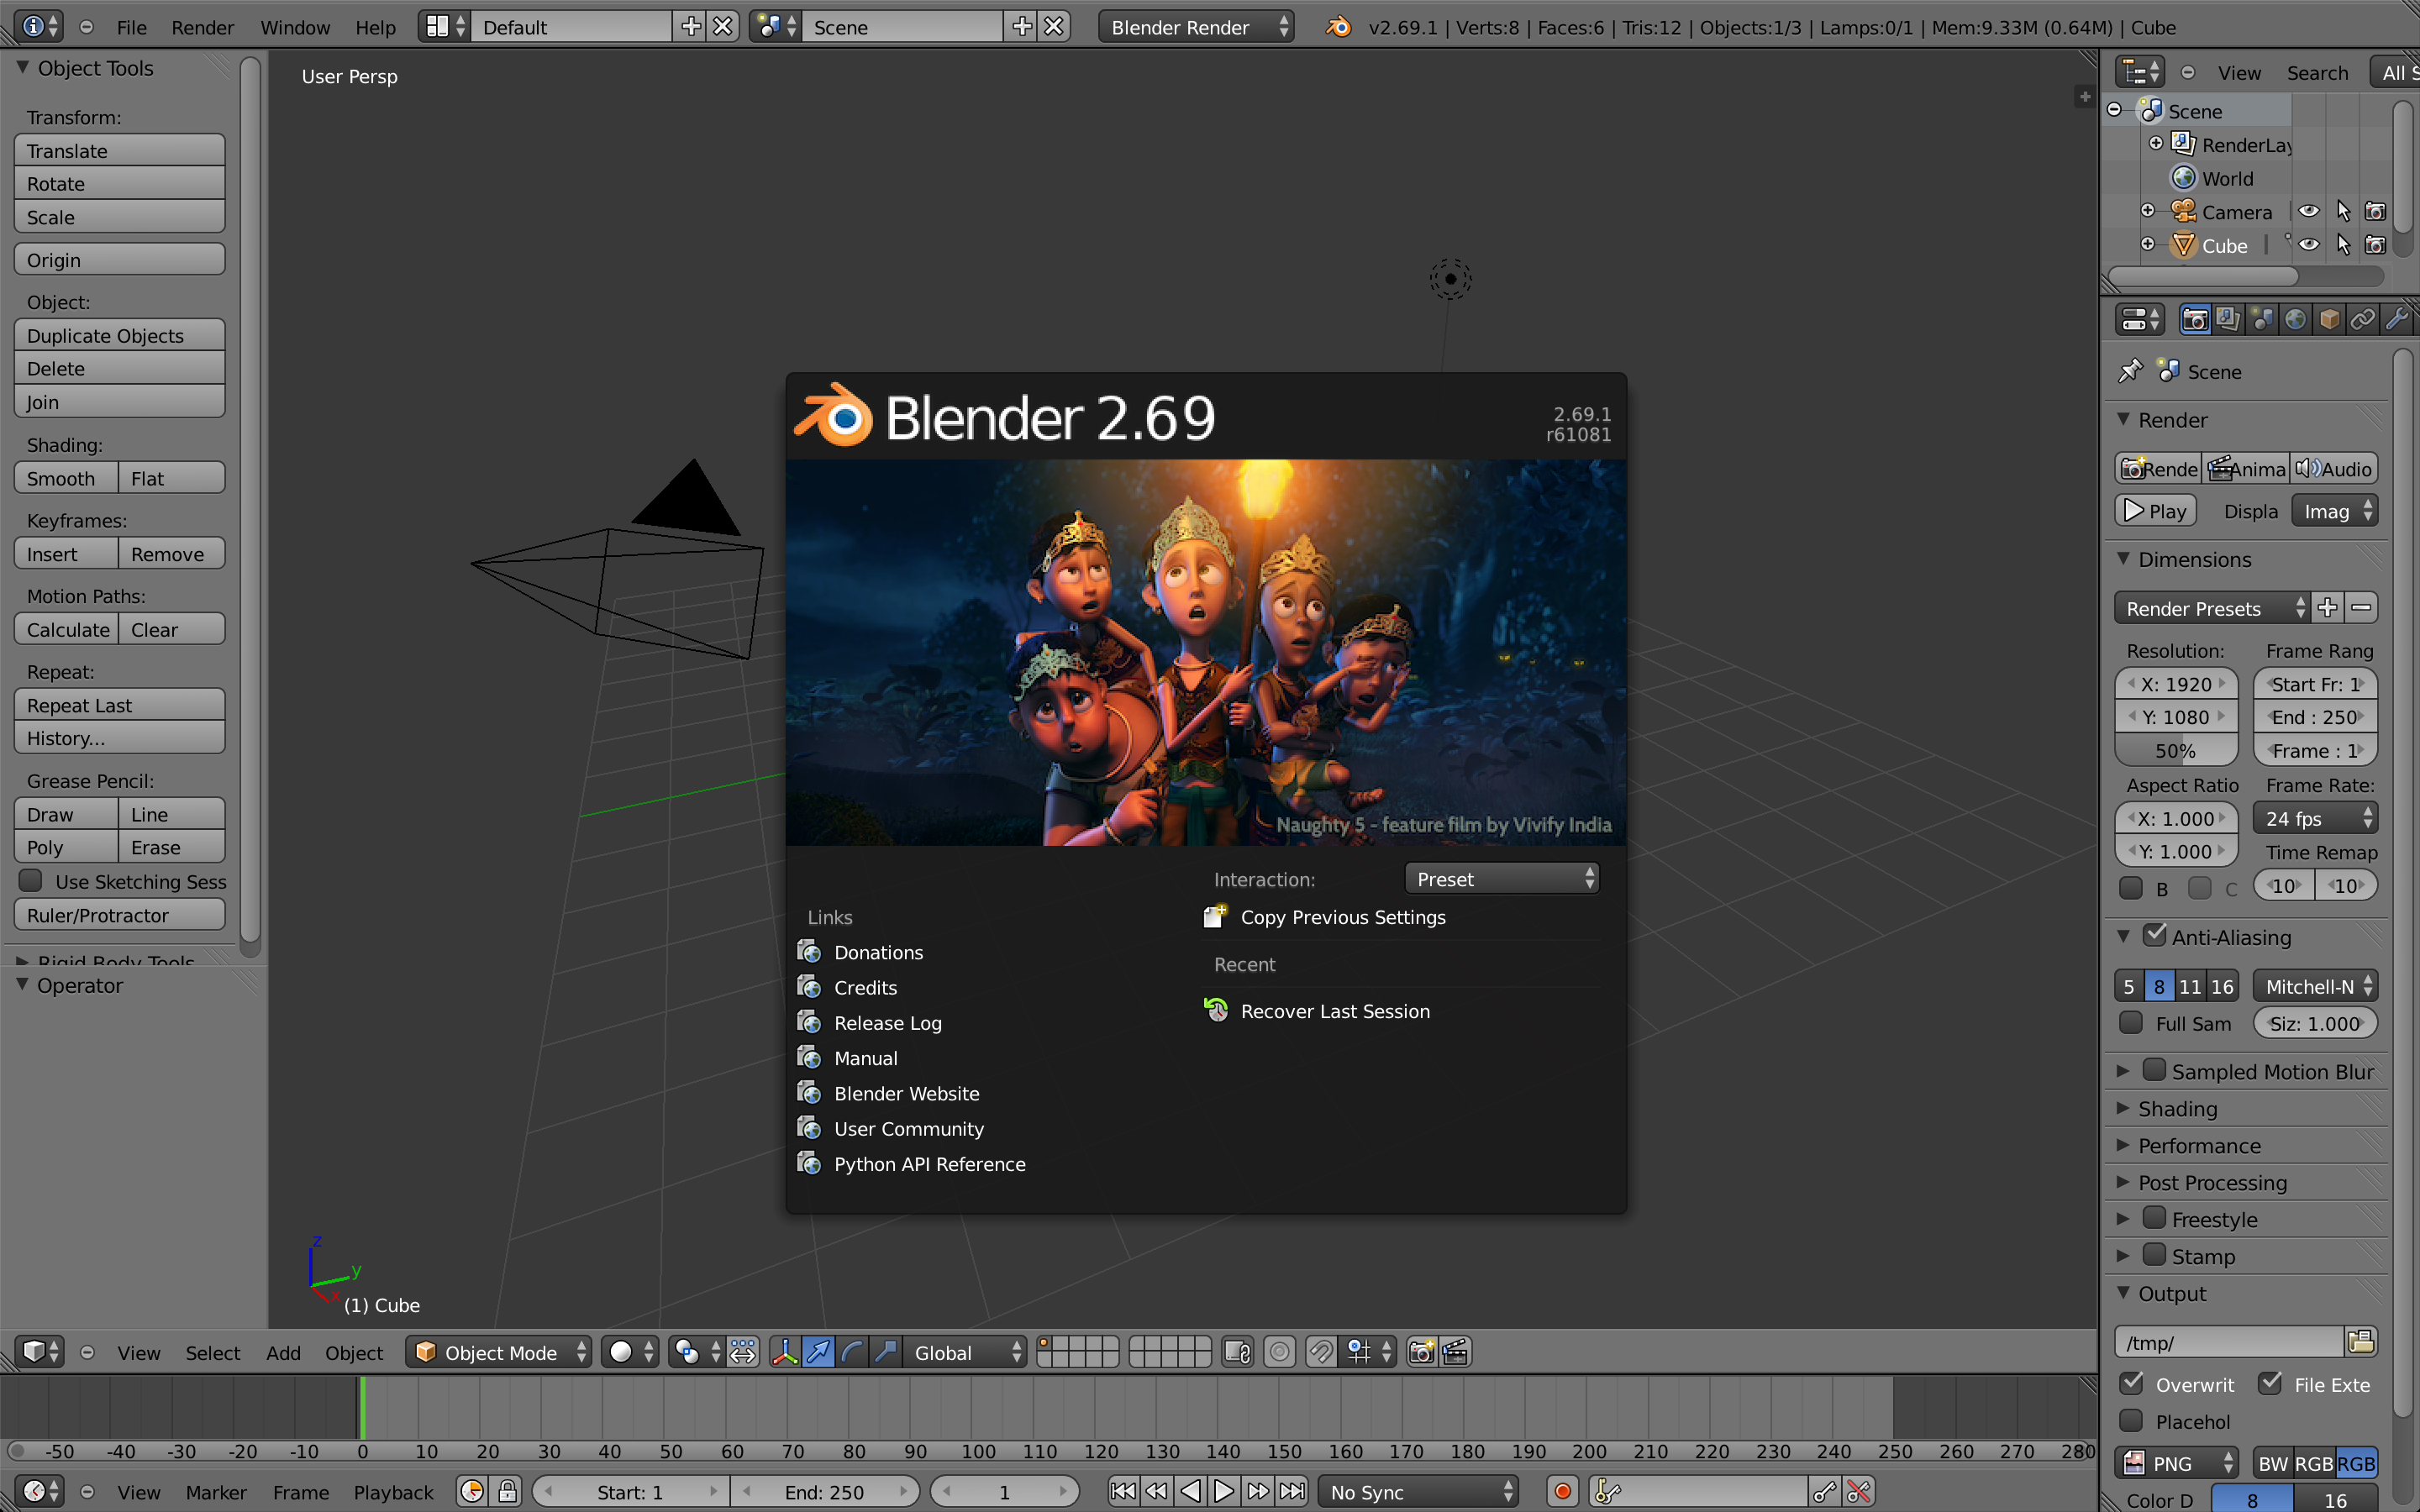
\includegraphics[width=17cm]{blender_gui}
\caption{Interface do Blender, ao abrir a aplicação.}
\label{blender_gui}
\end{figure}

Os principais módulos do Blender são implementados em C, sendo que camadas mais altas usam C++, como a interface gráfica (GUI), que usa OpenGL para não depender dos servidores gráficos de cada plataforma. Os projetos criados no Blender são salvos em arquivos {\it *.blend}, que salvam metadados em cabeçalhos, também a fim de permitir a compatibilidade entre arquiteturas diferentes. Exemplos de metadados salvos são tamanhos de ponteiros, versão do software, e disposição de memória\footnote{Exemplos são {\it little endian} e {\it big endian}.}.

Após o cabeçalho do arquivo, blocos de dados são salvos com informações como códigos identificadores dos objetos na cena, tamanho em memória dos objetos e índices das estruturas de dados que compõe a cena. Cada um destes blocos possuem os vetores de dados com os nomes e tipos de cada objeto, como curvas, malhas, luzes, câmeras, entre outras possibilidades.  

\subsection{Renderização no Blender}

Como o Blender é estruturado de maneira bastante modular, a renderização de uma cena criada no \emph{software} pode ser feita por {\it engines} diferentes, a escolha do usuário. Em uma instalação convencional, o Blender oferece duas \emph{engines} diferentes, mas há suporte para renderizadores de terceiros, com diferentes níveis de integração. \\

As duas \emph{engines} fornecidas são a {\it Blender Internal Render}, às vezes chamada apenas de {\it Blender Render} e o {\it Cycles}.
Elas serão discutidas com maiores detalhes a seguir. Na Figura \ref{renderers}, é mostrado onde, na interface do Blender, a opção por uma engine ou outra pode ser feita. Uma terceira engine, a {\it Blender Game Engine}, também é fornecida, mas engloba muito mais que apenas a geração de imagens, e é usada para a criação de games ou de aplicações interativas, gerando um arquivo executável como resultado. \\

%figura aqui!! :-P
\begin{figure}[!htb]
\center
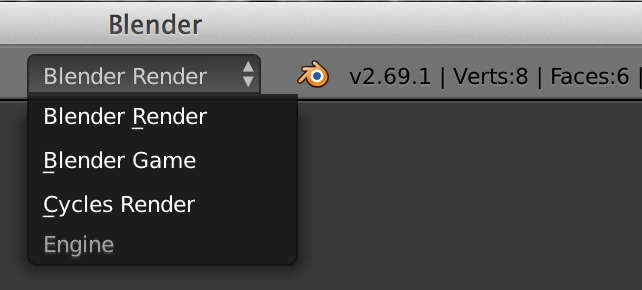
\includegraphics[width=8cm]{blender_render_option}
\caption{Interface do Blender, que permite a escolha de qual engine usar para renderização da cena.}
\label{renderers}
\end{figure}

É possível pré-visualizar a cena, animada ou estática, nas {\it viewports} da aplicação, e estas podem ser em {\it (i)} {\it wireframe}, mostrando apena as arestas dos objetos, {\it (ii)} sólida, preenchendo as superfícies com uma estratégia de {\it shading} simplificada para rápida visualização, ou ainda {\it (iii)} com texturas, permitindo uma visualização mais próxima do resultado final, porém mais lenta de ser obtida e menos interativa, já que o tempo de resposta da interface cai consideravelmente. Quando uma renderização completa e de qualidade final é necessária, todo o modelo de dados do Blender é passado à engine de renderização escolhida, software que, conforme discutido, calcula a emissão, absorção, reflexão e transporte da luz simulada e projeta os resultados sobre um plano de imagem definido pela câmera colocada em cena.

\subsubsection{Blender Internal Render}

A primeira geração de renderizador incluído no Blender, bastante estável, é útil para a geração de imagens em geral, com suporte a renderização volumétrica e a uso da GPU para os cálculos. Esta engine não é fisicamente fiel\footnote{{\bf Fisicamente fiel}, neste contexto, significa que os fundamentos usados para a geração de imagens são as leis da física e suas expressões matemáticas. Unidades e conceitos físicos são usados nos algoritmos e as imagens computadas são ditas fisicamente corretas, isto é, elas correspondem ao comportamento da luz que seria encontrado numa cena real.}, isto é, as unidades e grandezas usadas nas configurações podem usar, e normalmente usam, valores irreais para quantidades de luz. Um exemplo: uma superfície pode refletir 110\% da luz incidente, mesmo quando não é uma superfície emissora de luz.

\subsubsection{Cycles Render}

É uma engine mais moderna, fisicamente fiel, que modela efeitos cáusticos de maneira realista. Tem suporte a configuração de comportamento através de nós e permite que o usuário crie seus próprios shaders em OSL, linguagem apresentada em \ref{osl}. Um exemplo de uma rede de nós para configurar seu comportamento é mostrado na Figura \ref{nodes}. \\

%figura aqui!! :-P
\begin{figure}[!htb]
\center
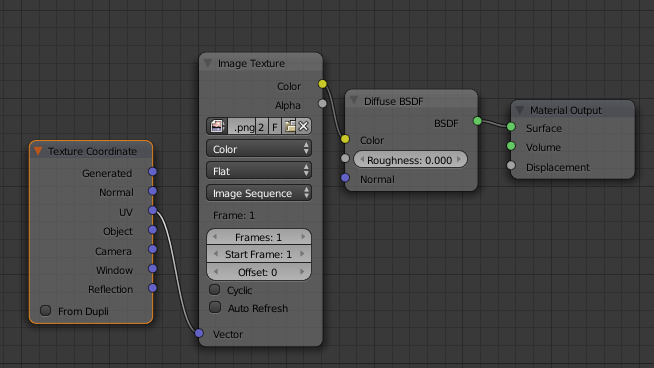
\includegraphics[width=15cm]{Cycles_nodes}
\caption{Rede de nós configurando o uso de uma sequência de imagens como textura para uma superfície.}
\label{nodes}
\end{figure}

Como o software é recente, ele é menos estável e nem todas as funcionalidades desejadas estão disponíveis. Uma das funcionalidades pendentes de implementação é a renderização de volumes, ou volumétrica, assunto deste trabalho.

\section{Texturas}
\label{tex_def}

No processo de modelagem tridimensional, a medida que detalhes se tornam mais sofisticados e complexos, a modelagem explícita de todas as informações desejadas, seja pelo uso de polígonos ou de outras primitivas geométricas, se torna pouco prático e de difícil execução. Uma alternativa é mapear uma imagem à superfície, técnica denominada {\it Mapeamento de Textura}. A imagem utilizada é chamada de {\it textura} e os elementos individuais que compõem a textura são chamados de {\it texels} (\emph{texture elements}, a exemplo do que ocorre com \emph{pixels}). Na imagem resultante, é usual que um \emph{pixel} contenha vários \emph{texels}.

\subsection{Definição}

Textura é um termo bastante amplo em síntese de imagens. De modo geral, podemos dizer que sempre que um ponto é avaliado usando apenas informações locais àquele ponto, trata-se de uma textura. Estas informações locais podem ser a localização do ponto no espaço, sua posição numa superfície, a direção e módulo das derivadas parciais da superfície naquele ponto, entre outras possibilidades. A função avaliada no ponto normalmente retorna um escalar, mas este resultado poderia, a princípio, ser de qualquer tipo, incluindo um vetor ou uma cor. É bastante usual que texturas sejam usadas como parâmetros de funções de {\it shading}.

Uma {\it textura volumétrica} pode ser avaliada em qualquer ponto do espaço; uma {\it textura de superfície} pode ser avaliada apenas sobre os pontos pertencentes à superfície. Além disso, texturas podem ser geradas por um programa e avaliadas sob demanda, ou armazenadas em um arquivo e consultadas para encontrar o valor da textura.

O {\it Mapeamento de Textura}, discutido na próxima seção, descreve a aplicação de uma textura a uma superfície, e determina a relação entre a geometria e o processo de {\it shading}.

\subsection{Mapeamento de Textura}

As texturas são introduzidas nas imagens com o uso de {\it mapeamentos de textura}. É uma forma de adicionar detalhes às superfícies sem que exista um modelo geométrico destes detalhes, de modo a permitir a criação de imagens complexas sem causar um aumento de complexidade na geometria.

De modo geral, mapas de texturas podem ser funções de uma ou mais variáveis. A fim de exemplificar seu funcionamento, mostraremos o caso das funções de duas variáveis.

Um \emph{mapa de textura} associa um {\it texel} a cada ponto no objeto geométrico. Se o objeto for representado por coordenadas homôgeneas, as funções serão dadas por:
\[
	\begin{array}{l}
	x = x(s, t), \\
	y = y(s, t), \\
	z = z(s, t), \\
	w = w(s, t).
	\end{array}
\]

Embora estas funções existam conceitualmente, encontrá-las pode ser difícil. Além disso, o problema mais usual é o inverso: dado o ponto $(x,y,z)$ ou $(x, y, z, w)$ no objeto, desejamos encontrar as coordenadas de textura correspondentes, isto é, as funções inversas 
\[
\begin{array}{l}
s = s(x, y, z, w), \\
t = t(x, y, z, w).
\end{array}
\]

Em computação gráfica, a maioria das superfícies são representadas parametricamente. Um ponto ${\bf p}$ na superfície é uma função de dois parâmetros $u$ e $v$. Para cada par de valores, geramos o ponto

\[
{\bf p}(u,v) = \left[ \begin{array}{c} x(u,v) \\ y(u,v) \\ z(u,v) \end{array} \right].
\]    

Dada uma superfície paramétrica, podemos mapear um ponto do mapa de textura $T(s,t)$ para um ponto ${\bf P}(u,v)$ na superfície usando um mapa linear da forma
\[ \begin{array}{l}
 u = as + bt + c, \\
 v = ds + et + f.
 \end{array}
\]

Neste conjunto de equações, $a$, $b$, $c$, $d$, $e$ e $f$ são coeficientes que definem o mapeamento linear. E se tivermos que $ae \neq bd$, este mapeamento é invertível. 

%figura aqui!! :-P
\begin{figure}[!htb]
\center
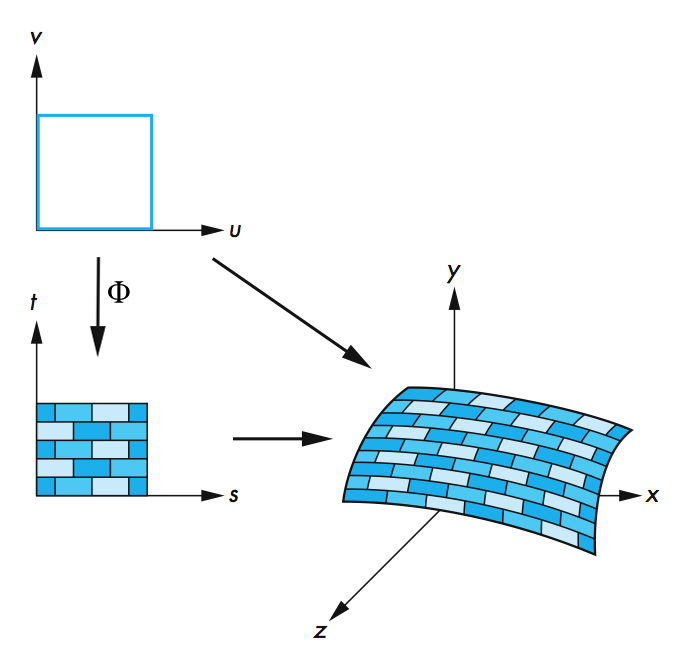
\includegraphics[width=11cm]{tex_mapping}
\caption{Mapeamento do sistema de coordenadas da região parametrizada para o sistema de coordenadas da textura.}
\label{tex_map}
\end{figure}

\subsubsection{Coordenadas de Textura}

Depois de a textura ter sido carregada na memória, ela pode ser amostrada, a fim de se obter uma cor a partir dela. Isso é feito usando \emph{coordenadas de textura}. Usualmente são atributos dos vértices, como posição e cor, armazenados como vetores, que determinam a distância em cada eixo da textura em que a amostra deve ser tomada. o tamanho do vetor depende do número de dimensões que a textura tem - uma textura 2D usa um vetor de pares ordenados para as coordenadas, por exemplo. Estas coordenadas são normalizadas, isto é, independente do tamanho da textura em uso, suas coordenadas variam entre $[0.0, 1.0]$. Como resultado, a aplicação não precisa se preocupar com o tamanho da textura depois que ela foi lida. 

\subsection{Estratégias de \emph{Wrapping}}
Embora texturas sejam definidas como tendo coordenadas normalizadas, os vértices podem usar coordenadas fora deste intervalo. O que ocorre neste caso depende do modo escolhido para {\it wrapping} da textura, que basicamente se refere a como a textura vai ``embrulhar'' a geometria. Um dos modos é denominado \emph{clamping}, que limita os {\it texels} ao tamanho da textura, isto é, se a coordenada solicitada é maior que a textura, a consulta vai retornar o valor da fronteira mais próxima da textura, efetivamente limitando o intervalo válido de consulta ao intervalo $[0.0, 1.0]$. No entanto, se a repetição da textura for permitida, as coordenadas para consulta à textura fazem um \emph{loop} na textura: solicitar o valor da textura no ponto $1.5$, $2.5$ ou até mesmo $100.5$, retorna o valor referente ao meio da textura, de coordenada $0.5$ no eixo considerado. \\

Na API adotada para este trabalho, a estrutura \texttt{Wrap} define os métodos suportados, como mostrado no Código \ref{wrap_enum}. O modo \emph{Black} retorna a cor preta pra qualquer ponto que caia fora do intervalo normalizado, isto é, todo ponto que estiver fora da área da textura, recebe a cor preta como resultado. O modo \emph{Clamp} limita todas as consultas para o intervalo da textura, e retorna o valor da extremidade mais próxima quando o ponto solicitado estiver além da fronteira da textura. Os modos \emph{Periodic} e \emph{Mirror} repetem a textura, sendo que o primeiro repete a textura em sua orientação normal e o segundo reflete a textura em relação a um dos eixos antes de repeti-la.

\begin{figure}[!htb]
\lstinputlisting[label=wrap_enum,caption={Modos de {\it wrapping} suportados pela API.}]{sourceCode/wrap_enum.cpp}
\end{figure}

\subsection{Texturas Tridimensionais}
\label{texturas3d}

A renderização volumétrica (chamaremos de renderização volumétrica o processo de geração de imagens que use uma textura tridimensional) parte da existência de um campo escalar contínuo tridimensional, que pode ser escrito como um mapeamento
\[ \Phi : \mathbb{R}^{3} \rightarrow \mathbb{R},
\]
que é uma função do espaço 3D para um valor de apenas um componente.
Na prática, um campo volumétrico é dado por uma imagem tridimensional, pois trata-se do resultado de uma simulação ou de uma medição. A Figura \ref{grid_ex} mostra um \emph{grid} bidimensional e outro tridimensional, exemplificando os dados para os campos escalares discretos e uniformemente amostrados.

%figura aqui!! :-P
\begin{figure}[!htb]
\center
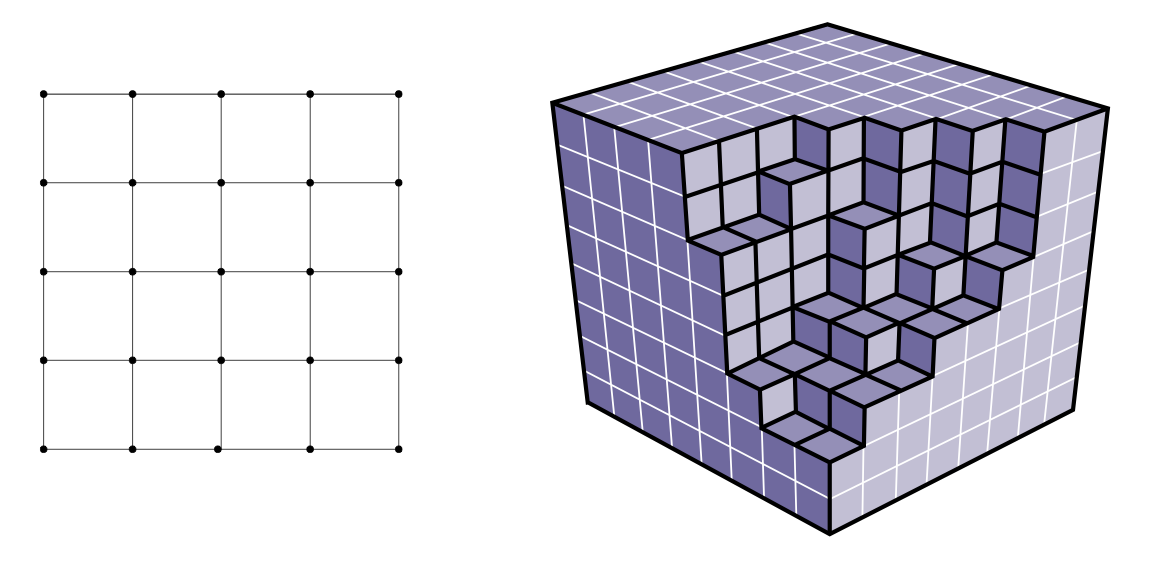
\includegraphics[width=11cm]{grid_example}
\caption{Exemplos de \emph{grids} uniformes: bidimensional com células de razão de aspecto 1, à esquerda, e tridimensional com células cubóides, à direita.}
\label{grid_ex}
\end{figure}

Uma imagem digital bidimensional é um bom exemplo para discutirmos a representação de um volume. Uma imagem consiste de {\it pixels} (abreviação de {\it picture elements}, elementos da figura, em inglês) organizados em um vetor convencional. {\it Pixels} são os elementos de dados de uma imagem 2D, e que possuem valores de cor.
Um conjunto volumétrico discreto pode ser representado de uma maneira similar se levarmos o espaço de duas para três dimensões. Assim, um \emph{pixel} 2D passa a ser um {\it voxel} 3D ({\it volume element}, elemento de volume, em inglês). {\it Voxels} são organizados em um vetor tridimensional convencional também, abrangendo o conjunto de dados que compõe o volume.
Embora seja intuitivo, o termo {\it voxel} tem duas possíveis interpretações. A primeira delas é a de que o {\it voxel} é um pequeno cubo que preenche uma pequena região volumétrica com o valor a ser armazenado. A outra interpretação assume que os {\it voxels} são pontos no espaço de três dimensões, ou seja, sem dimensão, sendo necessário o uso de técnicas de interpolação para preencher os espaços intermediários entre os pontos. Neste trabalho, esta última interpretação se adequa melhor, dada a biblioteca que usamos para representar volumes e as estratégias implementadas para reconstruir os valores nas lacunas entre os pontos definidos. \\

Um \emph{grid} uniforme $n$-dimensional tem a vantagem de ser bem estruturado, o que leva a uma representação compacta na memória do computador (na forma de um vetor $n$-dimensional) e acesso rápido, constante $O(1)$, às celulas. Porém, conforme será discutido no Capítulo \ref{data_struct}, essa representação só é eficiente para os casos em que o volume é denso, isto é, não há predominância de células intermediárias vazias. Além disso, \emph{grids} uniformes não são muito flexíveis, e outras estruturas de volumes podem ser usadas em seu lugar, sendo que apresentaremos uma das possibilidades. \\

\subsubsection{Voxels}

Conforme discutido na seção anterior, podemos acessar o conteúdo de um \emph{voxel} usando suas coordenadas no espaço, da mesma forma que podemos acessar o conteúdo de uma imagem bidimensional. É usual chamarmos as variáveis que representam os índices de $i$, $j$ e $k$ para os eixos $x$, $y$ e $z$, respectivamente. Em notação matemática, é comum a opção por índices subscritos, por exemplo: para um buffer de \emph{voxels}  $B$, dizemos que ele possui \emph{voxesl}  nos pontos amostrais dados por $B_{i,j,k}$. Na implementação, os dados amostrados são acessados usando coordenadas com sinal. Um exemplo é mostrado no Código \ref{vdb_coords}.

\begin{figure}[!htb]
\lstinputlisting[label=vdb_coords,caption={Consulta ao valor de ponto flutuante no voxel de coordenadas (1, 2, 3)}]{sourceCode/vdb_coordinates.cpp}
\end{figure}

\subsubsection{Fonte dos dados de uma textura volumétrica}

Os dados usados para a renderização volumétrica podem ser provenientes de diferentes áreas de aplicação. Um tipo importante de aplicação é a visualização científica de dados escalares. Mais especificamente, a visualização de imagens médicas é uma das aplicações mais proeminentes em visualização. Para obter os dados tridimensionais, usa-se equipamentos de escaneamento não invasivos, como  tomografia computadorizada ou ressonância magnética. \\

Outra fonte corriqueira de dados volumétricos são as simulações numéricas, como as simulações de dinâmica de fluidos, campos magnéticos e de fogo e explosões para efeitos especiais. Neste caso, o \emph{grid} usado para a simulação é normalmente bem diferente daquele usado para visualização. O \emph{grid} usado na simulação pode ser estruturado para garantir uma simulação estável, com características específicas ao fenômeno modelado. \\

Aplicações de visualização normalmente dependem de um \emph{grid} uniforme, que facilita métodos rápidos de geração de imagens. Desta forma, é usual que grids resultantes de simulações sejam transformados antes de fornecidos a um renderizador volumétrico. 

\subsubsection{Reconstrução}

Como um conjunto volumétrico de dados é representado de forma discreta, existe o problema de reconstruirmos uma função escalar em todos os pontos do domínio 3D.
O problema de uma reconstrução fiel é estudado em processamento de sinais. \\

Pelo teorema de amostragem de Nyquist-Shannon da teoria da informação, temos que a frequência do sinal de entrada precisa ser maior que o dobro da frequência máxima que ocorre no sinal de entrada para que o sinal original possa ser reconstruído a partir do sinal amostrado. Caso contrário, o sinal apresentará problemas de serrilhamento (\emph{aliasing}), isto é, o sinal contínuo será reconstruído com erros a partir do sinal discreto. \\

Em notação matemática, a amostragem apropriada pode ser descrita da seguinte forma: para um sinal de entrada periódico e contínuo representado pela função $f(t)$, determinamos primeiro sua frequência máxima $v_{f}$. Frequência máxima significa que a transformada de Fourier de $f(t)$ é zero fora do intervalo de frequências $[-v_{f}, v_{f}]$. Com isso, temos a frequência crítica de amostragem (também chamada de frequência Nyquist) $v_{N} = 2v_{f}$. Para uma amostragem apropriada, mais que $2v_{f}$ amostras precisam ser tomadas por unidade de distância. Para uma amostragem uniforme numa frequência $v_{s}$, os pontos amostrais podem ser descritos por $f_{i} = f(i/v_{s})$, com $i$ inteiros. \\

Dado que o sinal original é amostrado numa frequência $v_{s} > v_{N}$, o sinal pode ser recuperado das amostras $f_{i}$ conforme abaixo:
\[
	f(t) = \sum_{i} f_{i}\;sinc(\pi (v_{s}t - i)).
\]

A função $sinc(x)$ (de {\it sinus cardinalis}, seno cardinal, em latim) é dada por:
\[
	sinc(t) = \left\{ 
	\begin{array}{cl} 
	\frac{sen(t)}{t} & se\;\; t \neq 0  \\
	1 & se\;\; t = 0
	\end{array} \right. 
\]

Um sinal cuja transformada de Fourier é zero fora do intervalo de frequências $[-v_{f}, v_{f}]$ é chamado de limitado em banda porque sua largura de banda (isto é, sua frequência) é limitada. Na prática, as frequências que ocorrem num dado conjunto de dados podem ser desconhecidas. Nestes casos, um filtro passa-baixa pode ser aplicado para restringir a frequência máxima em um valor controlado. \\

A $f(t)$ apresentada é um exemplo de convolução, e descreve a convolução do sinal amostrado de entrada $f_{i}$ com um filtro $sinc$. Na realidade, porém, o filtro $sinc$ possui alcance ilimitado, isto é, ele oscila em torno de zero sobre todo o domínio. Como consequência, a convolução precisa ser calculada para todas as amostras de entrada $f_{i}$, o que toma muito tempo. É por isso que na prática aplica-se filtros de reconstrução com suporte finito.

Um exemplo é o filtro {\it caixa}, que leva à interpolação do vizinho mais próximo quando a largura da caixa é igual à distância de amostragem (isto é, o valor da função reconstruída é dado pelo valor do ponto amostral mais próximo). Outro exemplo é o filtro {\it triangular}, que leva a uma reconstrução linear quando a largura de um lado for igual à distância de amostragem. A Figura \ref{filters} mostra três tipos diferentes de filtros de reconstrução que podem ser usados. \\

%figura aqui!! :-P
\begin{figure}[!htb]
\center
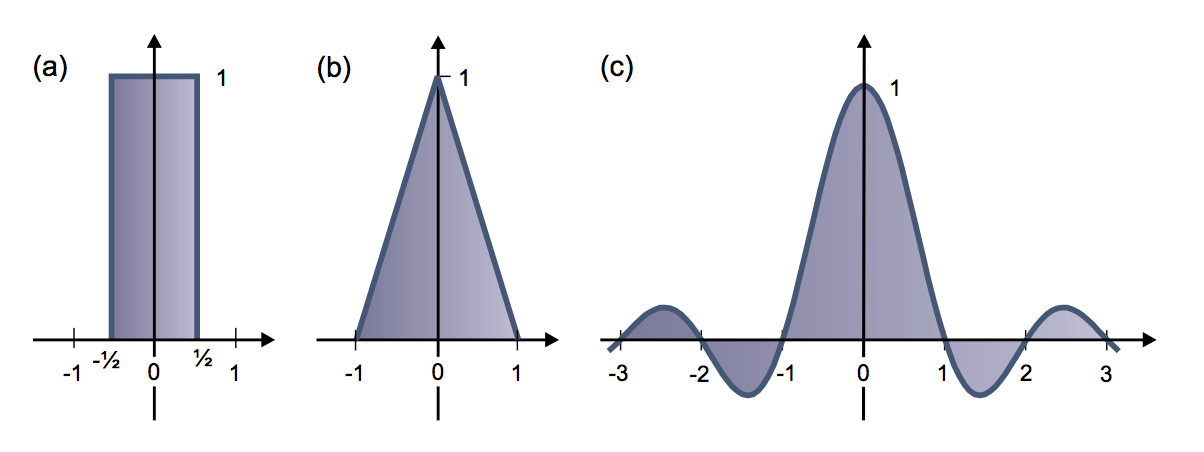
\includegraphics[width=15cm]{recon_filters}
\caption{Exemplos de filtros de reconstrução: (a) filtro caixa, (b) filtro triangular, e (c) filtros que usam o seno cardinal, {\it sinc}.}
\label{filters}
\end{figure}

Embora tenhamos discutido funções de apenas uma variável, podemos extender a discussão para $n$ dimensões usando uma abordagem de produto tensorial. A idéia é basicamente fazer a reconstrução de cada dimensão, mas de forma combinada. Para o nosso caso, em que precisamos de três dimensões, um filtro de reconstrução usando produto tensorial é dado por $h(x,y,z) = h_{x}(x)\;h_{y}(y)\;h_{z}(z)$, onde $h_{x}(\cdotp)$, $h_{y}(\cdotp)$ e $h_{z}(\cdotp)$ são filtros de um único parâmetro ao longo dos eixos $x$, $y$ e $z$. E uma das vantagens do uso de um \emph{grid} uniforme é que eles dão suporte a este tipo de reconstrução de forma direta. Como mostrado na Figura \ref{produtoTensorial}, a abordagem de produto tensorial separa as interpolações ao longo de cada dimensão e permite o cálculo do valor reconstruído através de uma sequência de interpolações lineares.

%figura aqui!! :-P
\begin{figure}[!htb]
\center
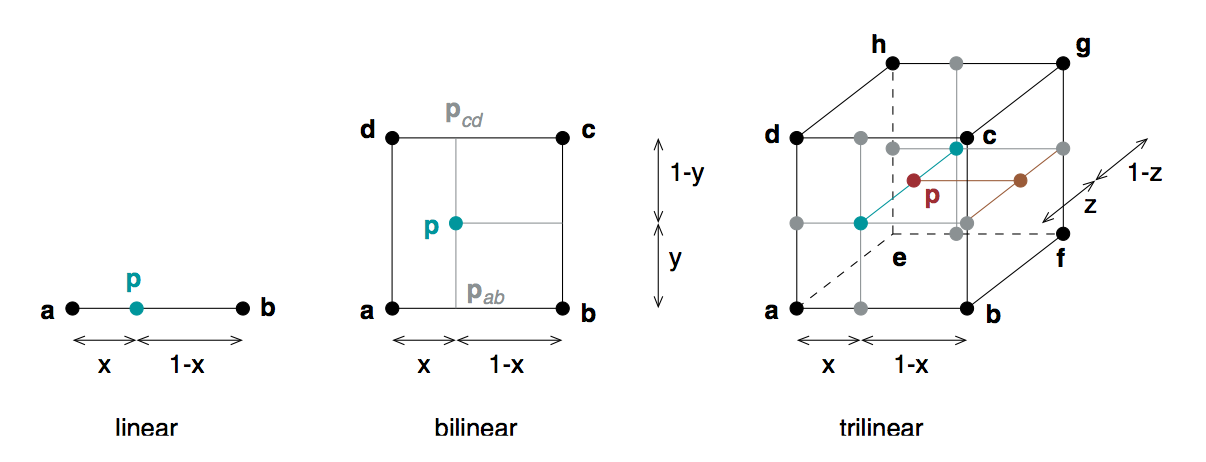
\includegraphics[width=15cm]{produtoTensorial}
\caption{Interpolações lineares usando o produto tensorial: casos linear, bilinear e trilinear.}
\label{produtoTensorial}
\end{figure}

\subsubsection{Filtros e Técnicas de Interpolação}

Quando desejamos aplicar uma textura 2D à superfície de uma geometria 3D, por exemplo, é bastante improvável que haja uma correspondência exata de $1:1$ entre os {\it texels} da textura e os {\it pixels} da tela ou da imagem a ser gerada. Duas possibilidades existem neste caso: quando uma textura é amostrada, o {\it texel} mais próximo do ponto solicitado pode ser retornado, ou uma \emph{interpolação} pode ser aplicada a um grupo de {\it texels} para que um valor possa ser calculado e retornado. \\

O exemplo mais simples de um filtro de textura no caso bidimensional é a \emph{Interpolação Bilinear} - os {\it texels} mais próximos nos eixos $x$ e $y$ são considerados a fim de calcular a cor final. \\

Para o caso de texturas tridimensionais, desejamos consultar o valor de um {\it voxel}. Pelo uso de coordenadas $(i, j, k)$ podemos acessar {\it voxels} individuais, mas a princípio, isso funciona apenas quando o ponto que desejamos amostrar corresponde exatamente ao centro do {\it voxel}. Em todos os outros casos, uma estimativa precisa ser feita acerca do valor, a ser definido pelos {\it voxels} vizinhos ao ponto que buscamos. As principais técnicas de interpolação serão discutidas a seguir. \\

\emph{Interpolação do vizinho mais próximo}. Em inglês, interpolação \emph{Nearest-Neighbor}. Trata-se da forma mais simples de interpolação, e pode-se dizer até que, de tão simples, não se qualifica como uma técnica de interpolação. Ao invés de considerar valores de {\it voxels} vizinhos, este método considera apenas o valor do centro do {\it voxel} que estiver mais próximo do ponto solicitado. Como consequência, a imagem resultante mostra claramente as fronteiras de cada {\it voxel}. 

Dada uma função discretamente amostrada {\bf d} e uma posição $x$, a interpolação do vizinho mais próximo em uma dimensão pode ser escrita como
\[
I_{n}(x, {\bf d}) = {\bf d}_{\floor*{x+0.5}}.
\]

Em código, temos um vetor unidimensional $A$ e uma coordenada de ponto flutuante $x$. Assumindo que $x$ está dentro do intervalo válido de $A$, a implementação é mostrada no Código \ref{nearestNeighbor}. O comportamento desta técnica de interpolação é ilustrado pela Figura \ref{nearestNeighborImage}. A implementação para o caso tridimensional é mostrado no código \ref{nearestNeighbor3d}. \\

\begin{figure}[!htb]
\lstinputlisting[label=nearestNeighbor,caption={Implementação da interpolação do vizinho mais próximo.}]{sourceCode/nearestNeighbor.cpp}
\end{figure}

%figura aqui!! :-P
\begin{figure}[!htb]
\center
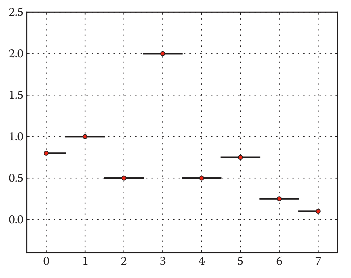
\includegraphics[width=9cm]{nearestNeighbor}
\caption{Interpolação do vizinho mais próximo. Os segmentos de reta mostram todo o intervalo que seria resolvido ao ponto denotado por cada círculo.}
\label{nearestNeighborImage}
\end{figure}


\begin{figure}[!htb]
\lstinputlisting[label=nearestNeighbor3d,caption={Implementação da interpolação do vizinho mais próximo para o caso tridimensional.}]{sourceCode/nearestNeighbor3d.cpp}
\end{figure}

\emph{Interpolação Linear}. Entre as técnicas de interpolação que usam valores intermediários para o cálculo, a interpolação linear é o caso mais simples. Os valores são calculados considerando os pontos próximos do ponto consultado e usando ponderação em função da distância, de modo que a contribuição de um ponto amostral é igual a $1.0$ se o ponto consultado está alinhado com o centro do voxel e é $0.0$ quando a distância do ponto consultado até o centro do voxel é $1.0$.

Dada a mesma função {\bf d} e coordenada $x$ do caso anterior, a interpolação linear pode ser escrita da seguinte forma:
\begin{center}
\[I_{l}(x, {\bf d}) = (1 - \alpha) \cdotp {\bf d}_{\left\lfloor x \right\rfloor} + \alpha \cdotp {\bf d}_{\left\lceil x \right\rceil}, \]
\[
\alpha = x - \left\lfloor x \right\rfloor.\]
\end{center}

A implementação é apresentada para o caso unidimensional no Código \ref{linear1d}. Para o caso tridimensional, há mais a ser feito. Os índices discretos precisam ser encontrados da mesma forma que no caso da interpolação pelo vizinho mais próximo, mas ao contrário daquele caso, precisamos agora dos valores de oito \emph{voxels} vizinhos, ao invés de apenas um. De modo geral, quanto maior a vizinhança que precisa ser considerada na interpolação, mais lento o processo. Definimos como \emph{Suporte} (denotado por $S$) o número de vizinhos a serem considerados numa dada técnica de interpolação. Para interpolação linear, temos $S = 2$. O número de valores de \emph{voxel} que uma técnica de interpolação precisa é dado por $2^{n}$, em que $n$ é o número de dimensões. Logo, para nosso caso, interpolação linear em três dimensões, o número de amostras necessário é $2^{3} = 8$. Na Figura \ref{linearInterp}, pode parecer que as descontinuidades indicam as fronteiras dos \emph{voxels} considerados, mas na realidade, a descontinuidade ocorre quando o ponto sendo amostrado passa de um intervalo $[r_{i-1}, r_{i}]$ para um intervalo $[r_{i}, r_{i+1}]$, e isso ocorre nos centros dos \emph{voxels}, e não nas fronteiras.

\begin{figure}[!htb]
\lstinputlisting[label=linear1d,caption={Implementação da interpolação linear para uma dimensão.}]{sourceCode/linear1d.cpp}
\end{figure}

%figura aqui!! :-P
\begin{figure}[!htb]
\center
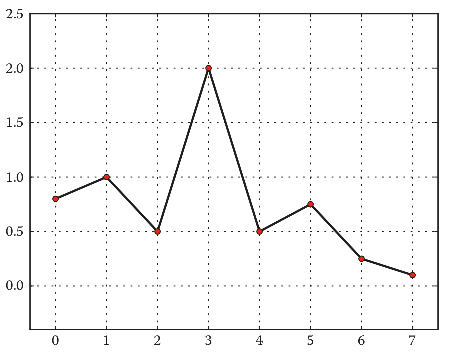
\includegraphics[width=9cm]{linear}
\caption{Interpolação linear. As quebras ocorrem na transição do centro de um voxel para o centro do voxel seguinte.}
\label{linearInterp}
\end{figure}

A implementação do caso tridimensional é apresentada no Código \ref{linear3d}. \\

%\begin{minipage}{\textwidth}
\begin{figure}[!htb]
\lstinputlisting[label=linear3d,caption={Implementação da interpolação linear para três dimensões.}]{sourceCode/linear3d.cpp}
\end{figure}
%\end{minipage}

\emph{Interpolação Cúbica}. A última técnica de interpolação que trataremos é a interpolação cúbica. A interpolação linear usa um polinômio de primeira ordem (linear) para calcular os valores intermediários, mas seu resultado, embora não seja ruim como a interpolação do vizinho mais próximo, ainda é pouco suave. Se usarmos polinômios de ordens maiores, obteremos resultados melhores, isto é, com transições mais suaves, ao custo de velocidade, já que o tempo de cálculo aumentará. 

O próximo passo, depois da interpolação linear, é a interpolação cúbica, que usa quatro valores vizinhos para a interpolação:
\[
 I_{c} (x, P_{i-1}, P_{i}, P_{i+1}, P_{i+2}).
\]  

Para derivar a fórmula da interpolação cúbica, consideramos a forma básica de um polinômio de terceira ordem e sua derivada:
\[
\begin{array}{l}
	f(x) = ax^3 + bx^2 + cx + d \\
f'(x) = 3ax^2 + 2bx + c.
\end{array}
\]
Os pontos que desejamos interpolar estão no intervalo $[0, 1]$, e os quatro pontos que funcionam como entrada para a função de interpolação são
\[
\begin{array}{rcl}
P_{i-1} & = & -1, \\
P_{i} & = & 0, \\
P_{i+1} & = & 1, \\
P_{i+2} & = & 2.
\end{array} 
\]

Calculando a função e sua derivada em $0$ e $1$, obtemos

\[
\begin{array}{rcl}
f(0) & = & d, \\
f(1) & = & a + b + c + d, \\
f'(0) & = & c, \\
f'(1) & = & 3a + 2b + c.
\end{array} 
\]

Reescrevendo cada um dos resultados de modo a isolar $a$, $b$, $c$ e $d$, obtemos
\[
\begin{array}{rcl}
a & = & 2f(0) - 2f(1) + f'(0) + f'(1), \\
b & = & -3f(0) + 3f(1) - 2f'(0) - f'(1), \\
c & = & f'(0), \\
d & = & f(0).
\end{array} 
\]

Sabemos os valores de $f(0)$ e de $f(1)$, mas os valores das derivadas não são dados diretamente à função. Porém, como temos $f(-1)$ e $f(2)$, podemos calculá-las:
\[
\begin{array}{rcl}
f(0) & = & P_{i}, \\
f(1) & = & P_{i+1}, \\
f'(0) & = & \frac{P_{i+1} - P_{i-1}}{2}, \\
f'(1) & = & \frac{P_{i+2} - P_{i}}{2}.
\end{array} 
\]

Combinando os dois últimos conjuntos de equações, encontramos os valores de $a$, $b$, $c$ e $d$ em sua forma simples e fechada:
\[
\begin{array}{rcl}
a & = & -\frac{1}{2}P_{i-1} +\frac{3}{2}P_{i} +\frac{3}{2}P_{i+1} +\frac{1}{2}P_{i+2}, \\
b & = & P_{i-1} +\frac{5}{2}P_{i} + 2P_{i+1} -\frac{1}{2}P_{i+2}, \\
c & = & -\frac{1}{2}P_{i-1} + \frac{1}{2}P_{i+1}, \\
d & = & P_{i},
\end{array} 
\]

o que nos leva à solução do problema original,


\begin{align*}
 I_{c} (x, P_{i-1}, P_{i}, P_{i+1}, P_{i+2}) = \left( -\frac{1}{2}P_{i-1} +\frac{3}{2}P_{i} +\frac{3}{2}P_{i+1} +\frac{1}{2}P_{i+2} \right)x^3 &+ \\
 \left( P_{i-1} +\frac{5}{2}P_{i} + 2P_{i+1} -\frac{1}{2}P_{i+2} \right)x^2 &+ \\ \left( -\frac{1}{2}P_{i-1} + \frac{1}{2}P_{i+1} \right)x &+ \\ P_{i}.
 \end{align*}

A interpolação cúbica usa dois valores abaixo e dois acima do ponto consultado, então a técnica tem um suporte $S = 4$, como é possível visualizar na Figura \ref{cubicInterp}. Em três dimensões, o custo total é dado por $4^3 = 64$ consultas para o cálculo de um único valor. No Código \ref{cubic}, a implementação é dada para uma, duas e três dimensões. A implementação de uma dimensão maior sempre usa a função definida para uma dimensão menor.

Uma das desvantagens da interpolação cúbica é que encontramos casos de {\it overshoots}. Quando temos grandes gradientes nos dados discretos, a técnica pode assumir valores maiores ou menores que qualquer um dos dados existentes em todo o conjunto. Dado o escopo deste trabalho, consideraremos que os problemas que isso acarreta são aceitáveis na geração de imagens para nossa aplicação.

%figura aqui!! :-P
\begin{figure}[!htb]
\center
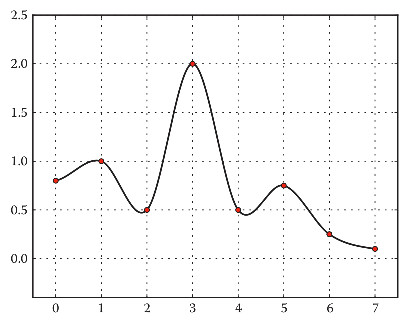
\includegraphics[width=9cm]{cubic}
\caption{Interpolação cúbica. Como o polinômio é de terceira ordem, as curvas são bem mais suaves que da interpolação linear.}
\label{cubicInterp}
\end{figure}

\begin{figure}[!htb]
\lstinputlisting[label=cubic,caption={Implementação da interpolação cúbica para uma, duas e três dimensões.}]{sourceCode/cubic.cpp}
\end{figure}

\section{Sistemas de Coordenadas}

É bastante natural que o conceito de Sistemas de Coordenadas permeie as aplicações de computação gráfica. Afinal, é bastante usual criar um objeto em seu próprio sistema de coordenadas, chamado de sistema de coordenadas de modelagem do objeto, e posteriormente colocar este objeto em uma cena usando as coordenadas do mundo. O objetivo principal de existirem vários sistemas de coordenadas é permitir uma execucação mais eficiente de cada passo do processo de visualização. Para este fim, os objetos precisam ser transformados para sistemas de coordenadas (ou espaços de referência) nos quais as tarefas inerentes a cada etapa do processo seja mais natural e conveniente. O processo gráfico completo, do modelo até a exibição da imagem em um monitor envolve o uso de 7 espaços diferentes. São eles os espaços do objeto, da cena ou do mundo, da câmera, espaço normalizado, de ordenação, de imagem e do dispositivo. Comentaremos apenas acerca dos dois espaços mais relevantes a esse trabalho, mas um tratamento completo pode ser encontrado em \cite{ANGEL}.

\subsubsection{Espaço do objeto}
Também chamado de espaço do modelo, é o sistema de coordenadas em que um objeto 3D específico está definido. Normalmente, embora não sempre, cada objeto terá seu próprio espaço de objeto com origem no centro do objeto em questão. Por centro, entenda-se o ponto em torno do qual o objeto é movido e rotacionado, como um pivô, e que pode não coincidir com o centro geométrico do objeto. Um exemplo é mostrado na Figura \ref{objectSpace}.

%figura aqui!! :-P
\begin{figure}[!htb]
\center
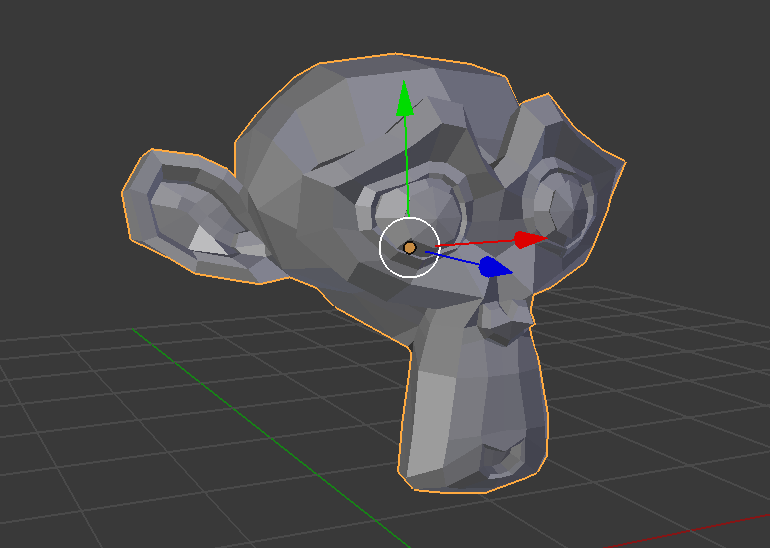
\includegraphics[width=7cm]{objectSpace}
\caption{Espaço do objeto.}
\label{objectSpace}
\end{figure}

\subsubsection{Espaço da cena}
Espaço da cena, também chamado de espaço do mundo, ou ainda de sistema de coordenadas global, é o sistema de coordenadas do universo tridimensional em consideração. Nele, os objetos do cenário são posicionados e orientados, uns em relação aos outros, incluindo a câmera virtual. Um exemplo é mostrado na Figura \ref{worldSpace}.


%figura aqui!! :-P
\begin{figure}[!htb]
\center
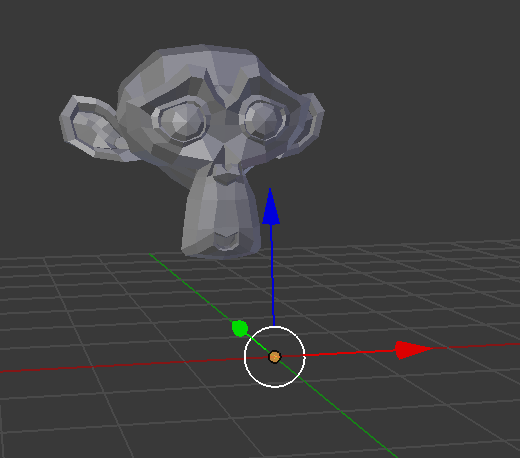
\includegraphics[width=7cm]{worldSpace}
\caption{Espaço da cena, com a origem centrada no círculo menor.}
\label{worldSpace}
\end{figure}

\subsection{Notação Homogênea}

Um ponto descreve um local no espaço, ao passo que um vetor descreve uma direção e não possui localização. Usando matrizes $3 \times 3$ (ou, eventualmente, $2 \times 2$ para duas dimensões), é possível aplicar transformações lineares como rotações, escala e cisalhamento às coordenadas. Contudo, translações não são possíveis com o uso destas matrizes. Essa característica não afeta operações com vetores, mas a translação é uma operação importante para pontos.


A notação homogênea é útil para transformar tanto vetores quanto pontos, e nos permite aplicar translações apenas aos pontos. As matrizes $3 \times 3$ são aumentadas para $4 \times 4$ e pontos tridimensionais e vetores passam a ter um elemento a mais. Assim, um vetor homogêneo é representado por ${\bf p} = (p_{x}, p_{y}, p_{z}, p_{w})$. Nestas condições, $p_{w} = 1$ para pontos e $p_{w} = 0$ para vetores. Quando lidamos com projeções, outros valores podem ser usados para $p_{w}$. Dessa forma, quando $p_{w} \neq 0$ e $p_{w} \neq 1$, precisamos homogeneizar o vetor, e fazemos $(\frac{p_{x}}{p_{w}}, \frac{p_{y}}{p_{w}}, \frac{p_{z}}{p_{w}}, 1)$ a fim de obter o ponto que de fato desejamos. No caso mais simples, $M$ é tal como mostrada abaixo.

\[ M_{4 \times 4} = \left(
\begin{array}{cccc}
m_{00} & m_{01} & m_{02} & 0 \\
m_{10} & m_{11} & m_{12} & 0 \\
m_{20} & m_{21} & m_{22} & 0 \\
0 & 0 & 0 & 1 
\end{array} \right)
\]

As matrizes específicas das transformações de rotação, escala e cisalhamento podem substituir a matriz $M$ apresentada, e estas operações afetarão pontos e vetores, como esperado. Uma translação, contudo, usa os elementos adicionais da matriz aumentada para obter o resultado necessário. Uma matriz de translação, $T$, que translada um ponto por um vetor $t$, é mostrada abaixo.

\[ T = \left(
\begin{array}{cccc}
1 & 0 & 0 & {\it t_{x}} \\
0 & 1 & 0 & {\it t_{y}} \\
0 & 0 & 1 & {\it t_{z}} \\
0 & 0 & 0 & 1 
\end{array} \right)
\]

A combinação de uma transformação linear seguida de uma translação é denominada {\it transformada afim}.

Verificamos com facilidade que um vetor ${\bf v} = (v_{x},v_{y},v_{z},0)$ não é afetado pela transformação ${\bf Tv}$ porque seu último elemento é 0. Se ao ponto $P= (P_{x},P_{y},P_{z},1)$ aplicarmos a transformada ${\bf T}P$, o resultado que obtemos é $P = (P_{x} + t_{x},P_{y} + t_{y},P_{z} + t_{z},1)$, ou seja, o ponto $P$ transladado por $t$.

Como é de se esperar, multiplicações entre matrizes e multiplicações entre matrizes e vetores são calculadas normalmente, sem alterar o que foi discutido.


\section{\emph{Shaders}}
\label{shaders}

Um \emph{shader} é um programa com entradas e saídas, que executa uma tarefa específica no processo de renderização de uma cena, como determinar a aparência de um material ou o comportamento de uma luz. O código fonte do programa é escrito em uma linguagem altamente dependente do ambiente alvo. Exemplos incluem a OpenGL Shading Language (GLSL) e a Direct3D High Level Shader Language (D3D-HLSL). Neste trabalho, a linguagem de \emph{shading} adotada é a Open Shading Language, discutida na Seção \ref{osl}.\\

De modo geral, \emph{shaders} são programas bastante simples que descrevem as características de um vértice ou de um \emph{pixel}. \emph{Shaders} de vértice descrevem as características de um vértice, como posição, coordenadas de textura, cores, entre outras características. \emph{Shaders} de \emph{pixel} descrevem informações como cor, profundidade (\emph{z-depth}, quando um \emph{z-buffer}\footnote{Algoritmo que implementa uma solução adotada para o problema de visibilidade tridimensional quando uma cena é transformada para as coordenadas de tela, e a profundidade relativa entre os objetos precisa ser estabelecida.} está sendo usado), transparência, entre outras possibilidades. 


\subsection{\emph{Open Shading Language}}
\label{osl}

A \emph{Open Shading Language} (OSL) é uma linguagem sucinta, apesar de bastante completa, para a programação de \emph{shaders} em renderizadores modernos e aplicações semelhantes, e é ideal para descrever materiais, luzes, deslocamentos e geração de padrões.
A linguagem foi desenvolvida pela Sony Pictures Imageworks para uso em seu renderizador proprietário para animação de longa-metragens e efeitos visuais. A especificação da linguagem foi desenvolvida com a participação de outras empresas produtoras de animação e efeitos especiais e que também possuíam interesse em utilizá-la.
A licença utilizada é a nova-BSD, de 1999, o que permite seu uso em qualquer aplicação gratuita ou comercial, aberta ou proprietária, bem como modificação do código fonte. \\

A OSL tem uma sintaxe parecida com a do C, e parecida também com outras linguagens de \emph{shading}. No entanto, ela foi escrita especificamente para algoritmos modernos de renderização e suporta \emph{closures}\footnote{Função ou referência a uma outra função, dotada de um ambiente de referência. Isto é, permite que uma função acesse variáveis não locais mesmo quando chamada fora de seu escopo léxico imediato.} para cálculo de cores, BSDFs\footnote{\emph{Bidirectional scattering distribution function}, função de distribuição bidirecional de propagação, em tradução livre. Trata-se da função que descreve como a luz é propagada por uma superfície.} e \emph{ray-tracing} postergado, com avaliação dos raios em momento posterior do processo de geração da imagem. \\

Uma das principais características desta linguagem é que o resultado dos \emph{shaders} de superfície e de volume são \emph{closures}, e não cores resultantes, o que seria mais habitual.
No entanto, temos que os \emph{shaders} escritos em OSL calculam uma descrição simbólica explícita, o \emph{closure}, para descrever como a superfície ou o volume propaga a luz, em unidades radiométricas. Estes \emph{closures} podem ser avaliados em mais de uma direção de propagação de luz, podem ser amostrados para encontrar direções importantes numa dada cena, ou armazenados para avaliação posterior pelo renderizador que está rodando o \emph{shader}. Esta abordagem é ideal para renderizadores que tentam ser fiéis ao comportamento físico da luz, especialmente para os que suportam \emph{ray-tracing}\footnote{Técnica de geração de imagens que se baseia em traçar raios de luz através dos \emph{pixels} no plano da imagem e simular os efeitos de suas interações com os objetos da cena modelada.} e iluminação global\footnote{\emph{Global Illumination} (GI) abrange as técnicas que consideram em adição à iluminação direta a iluminação indireta, como a reflexão da luz em outros objetos.}.


\begin{figure}[!htb]
\lstinputlisting[label=osl_struct,caption=Estrutura de um shader escrito em OSL.]{sourceCode/osl_structure.cpp}
\end{figure}

\chapter{OpenVDB}
\label{data_struct}


A estrutura de dados utilizada neste trabalho para a representação de volumes é a VDB, renomeada para OpenVDB\footnote{www.openvdb.org} na ocasião em que foi disponibilizada com código fonte aberto. OpenVDB é uma biblioteca que inclui uma estrutura de dados compacta e hierárquica e um conjunto de ferramentas para a manipulação eficiente de dados volumétricos discretizados esparsos, que podem variar com o tempo, em um \grid tridimensional. \\

A estrutura de dados foi desenvolvida pela DreamWorks Animation\footnote{www.dreamworksanimation.com}, e oferece um espaço de índices de três dimensões virtualmente infinito, armazenamento compacto, tanto na memória quanto em disco, acesso rápido aos dados, tanto sequencial quanto aleatório, e uma coleção de algoritmos otimizados especificamente para esta estrutura de dados para tarefas usuais como a aplicação de filtros, discretização de equações diferenciais parciais, conversão de polígonos em \voxels, e amostragem. Os detalhes técnicos da estrutura de dados e de sua manipulação são discutidos nas seções seguintes.

\section{Definição}
A biblioteca OpenVDB é composta pela estrutura de dados e pelo conjunto de ferramentas para a manipulação da estrutura. Muito embora haja grande interdependência entre estes dois itens, abordaremos cada item separadamente.

\subsection{A Estrutura de Dados VDB}
\label{vdb_data}

Uma das principais idéias em que a VDB se baseia é em organizar dinamicamente os blocos de dados de um \grid em uma estrutura de dados hierárquica semelhante a uma árvore B+. Essa semelhança é abordada na seção \ref{bplus_trees}. Estes blocos são folhas\footnote{{\bf Folhas}, ou nó-folha, são os nós de uma estrutura de árvore que não possui filhos e que assim diferem da raiz e dos nós internos.} que sempre ficam em uma mesma profundidade de um grafo conectado e acíclico com fatores grandes, e variáveis, de ramificação, sendo que os fatores de ramificação são necessariamente potências de dois. Isso implica que a árvore é balanceada em altura por construção, mas baixa e larga. Como resultado, temos um domínio mais amplo, e devido à altura baixa da árvore, o número de operações de E/S necessárias para percorrer a árvore da raiz até uma das folhas é menor. \\
  
\texttt{Templates} C++ são usados frequentemente na construção da estrutura, bem como funções \texttt{inline}, e funções virtuais são evitadas a todo custo. Trata-se de um pequeno conjunto de otimizações que, entre outras coisas, viabiliza o acesso aleatório rápido. Mais especificamente, as classes que implementam os diferentes nós da árvore são recursivamente geradas a partir de \texttt{templates} em função do tipo armazenado pelos filhos, ao invés de usar herança de uma classe base comum a todos os nós. A motivação para esta escolha é o fato de que os nós gerados a partir de \texttt{templates} são expandidos em linha (\texttt{inline}) durante a compilação, e com isso, as funções não possuem uma sobrecarga de execução, que ocorreria se a opção fosse pelo uso de herança.

Além disso, ao usarmos \texttt{templates}, fica mais fácil mudarmos a configuração de profundidade e ramificação da árvore, apesar de a escolha destas características precisar ser feita em momento de compilação, e não de execução. \\

Outras técnicas de implementação que contribuem ao desempenho da estrutura são operações \bit  a \bit, que são muito rápidas, armazenamento de informações usando \bits, uso do recurso de \texttt{union} do C++ para reúso de memória, e uso de execução paralela com suporte explícito a {\it threads} e operações SIMD\footnote{{\bf Single instruction, multiple data}, única instrução, dados múltiplos, em inglês, é uma classe de computadores paralelos na taxonomia de Flynn. Refere-se ao suporte de operações em que uma instrução é executada paralelamente em vários elementos de dados simultaneamente.}.

\subsubsection{Detalhes de implementação}
A VDB modela um espaço de índices $(x, y, z)$ infinito, embora na prática este seja limitado pela precisão de \bits da arquitetura e da memória disponível. Os dados armazenados na estrutura consistem em um tipo \texttt{Valor}, definido com o uso de \texttt{templates}, e em uma coordenada com os índices discretos $(x, y, z)$, especificando a localização espacial do ponto amostral, isto é, a {\it topologia} do {\it valor} dentro da estrutura da árvore. Conforme comentado anteriormente na Seção \ref{texturas3d}, a menor unidade de um elemento de volume será sempre chamada de \voxel. Um único {\it valor} é associado a cada \voxel, e cada \voxel pode existir em um de dois estados possíveis: {\it ativo} e {\it inativo}. A interpretação deste estado binário depende da aplicação que estiver usando a biblioteca, mas podemos considerar que os \voxels ativos são mais importantes, ou de maior interesse, para a aplicação. \\

A VDB armazena separadamente a {\it topologia} de um \voxel numa árvore cujo nó raiz cobre todo o espaço de índices e cujas folhas cobrem um subconjunto fixo do espaço de índices. Mais precisamente, a topologia é armazenada implicitamente em máscaras de \bit, e os valores associados a cada \voxel são armazenados de maneira explícita em buffers que podem estar localizados em qualquer nível da árvore - dizemos que a estrutura é multiníveis por isso. Áreas do espaço de índices em que todos os \voxels têm o mesmo valor podem ser representados com uma única entrada no nível correto da árvore. Assim como \voxels, os valores armazenados nos níveis intermediários da árvore também podem estar ativos ou inativos. O objetivo da VDB é usar o mínimo de memória possível para representar os \voxels ativos, mantendo as características de desempenho de uma estrutura de dados para volumes densos. \\

Um componente fundamental da estrutura de dados é o conjunto de máscaras de \bit incluídas nos vários nós da árvore, em diferentes níveis. O uso das máscaras de \bit permite acesso rápido e direto à representação binária da {\it topologia} local ao nó.  Um diagrama mostrando a estrutura interna da VDB é apresentado na Figura \ref{treeStructure}. \\

%figura aqui!! :-P
\begin{figure}[!htb]
\center
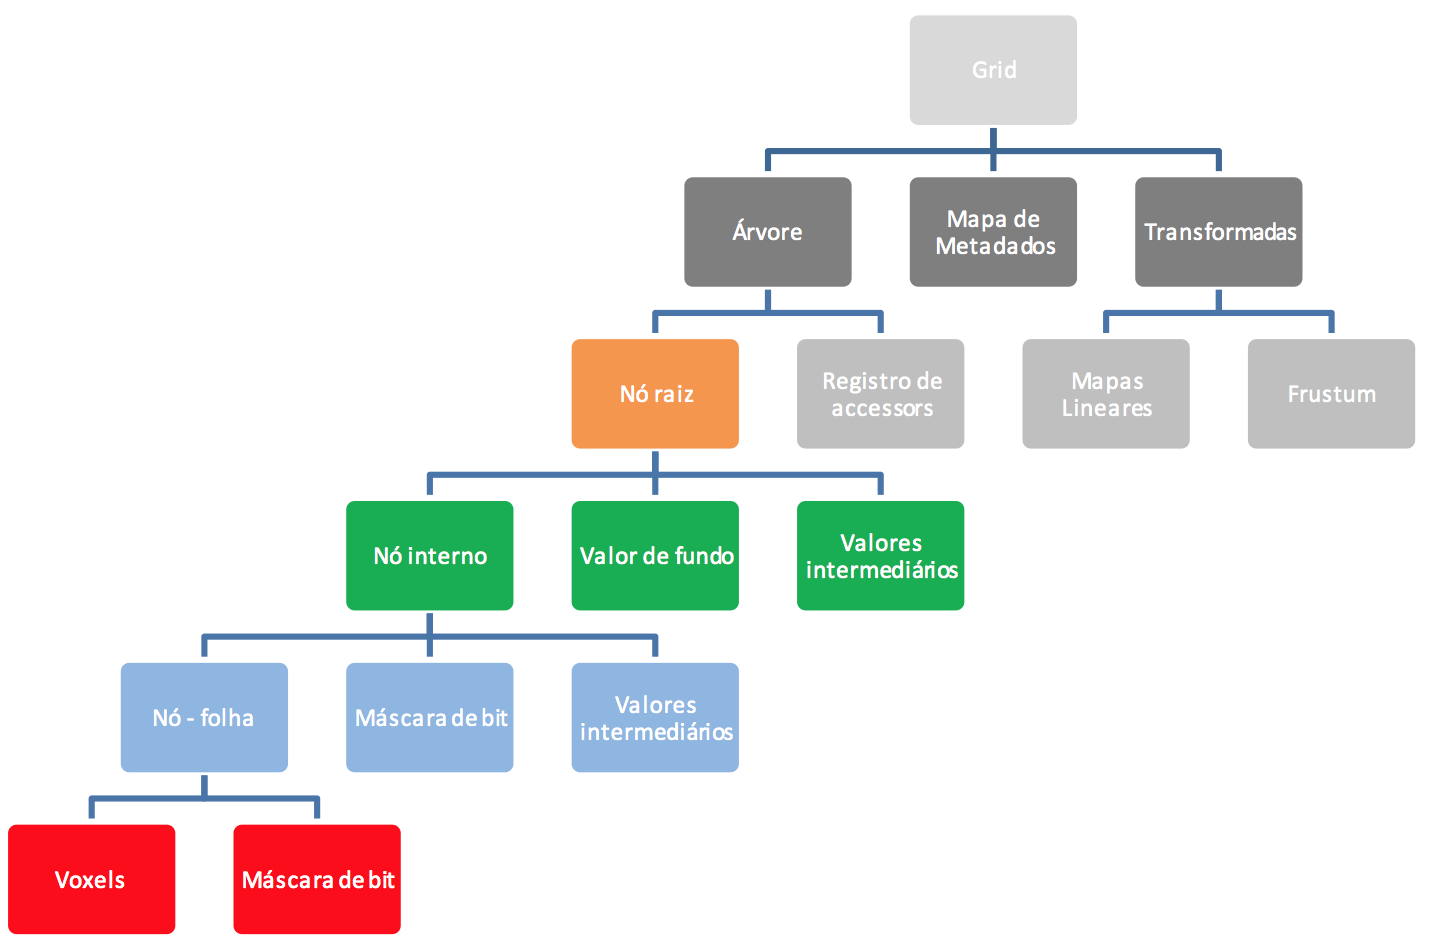
\includegraphics[width=16cm]{tree_structure}
\caption{Diagrama da estrutura interna da árvore VDB, conforme descrito em \cite{MUSETH}.}
\label{treeStructure}
\end{figure}

{\emph Folhas}. Estes nós são os blocos do \grid de nível mais baixo na estrutura e, por construção, todos estão na mesma profundidade da árvore. As folhas dividem o espaço de índices em subdomínios disjuntos com $2^{log_{2}(w)}$ \voxels em cada eixo, onde $2^{log_{2}(w)} = 1, 2, 3, ...$ e $w$ é qualquer entre $x$, $y$ ou $z$. Uma configuração típica, e recomendada, é estabelecer $2^{log_{2}(w)} = 3$, o que corresponde a um bloco $8 \times 8 \times 8$. As dimensões das folhas (e dos nós internos, que discutiremos a seguir) são restritas a potências de dois, pois isso permite as operações \bit a \bit com mais velocidade durante as buscas pela árvore.

\begin{figure}[!htb]
\lstinputlisting[label=leafNode,caption=Definição de um nó folha.]{sourceCode/leafNode.cpp}
\end{figure}

Como pode ser visto no Código \ref{leafNode}, os tamanhos são estabelecidos em momento de compilação, e o tamanho do nó é computado como $1 << \sum_{w} sLog_{2}(w)$, onde $<<$ denota um deslocamento de \bits à esquerda. As folhas armazenam os valores dos \voxels em uma tabela chamada de {\it Direct Access Table}\footnote{Pode-se assumir que esta tabela é um vetor com custo de acesso aleátorio de $O(1)$ para o pior caso.}, denotada no código por \texttt{mLeafDAT}, e a topologia do \voxel ativo é mantida na máscara de \bits denotada no código por \texttt{mValueMask}. É importante notar que embora a máscara de \bits tenha um tamanho fixo igual ao da estrutura \texttt{LeafNode}, o tamanho do vetor que armazena os valores dos dados é dinâmico, mantido em \texttt{mLeafDAT.values}. A quantidade variável de \buffers de dados, e seus tamanhos, bem como outras informações a respeito da \texttt{LeafNode} são armazenadas de forma compacta na varíavel de 64 \bits \texttt{mFlags}, mostrada na Figura \ref{mFlags}.

%figura aqui!! :-P
\begin{figure}[!htb]
\center
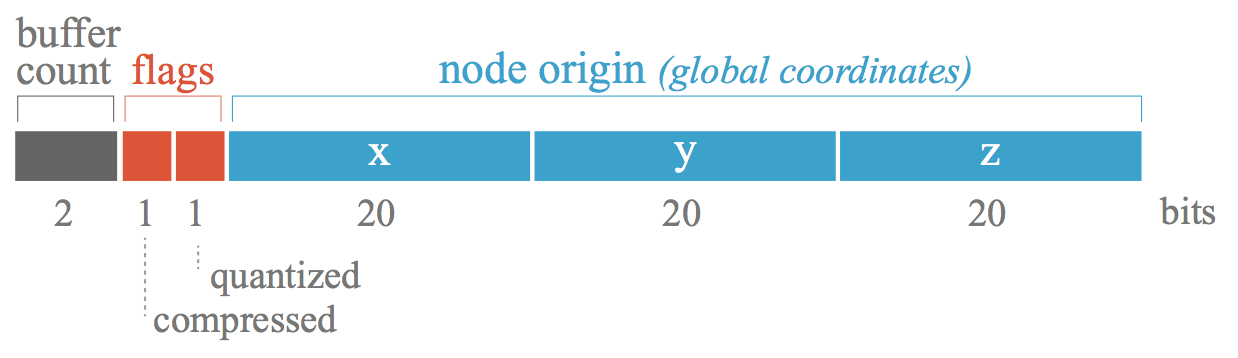
\includegraphics[width=12cm]{mFlags}
\caption{Representação compacta de \texttt{mFlags}, variável de 64 \bits que codifica: número de \buffers(2), compressão(1), quantização(1) e origem da folha ($3 \times 20$).}
\label{mFlags}
\end{figure}

Os primeiros dois \bits codificam um dos quatro estados possíveis: 0 \buffers, isto é, os valores são salvos externamente, 1 \buffer, valores salvos na memória sem suporte para integração em relação ao tempo, 2 \buffers, valores salvos na memória com suporte a integração em relação ao tempo de primeira e segunda ordem ou 3 \buffers, valores salvos na memória com suporte a integração em relação ao tempo de terceira ordem. O terceiro \bit é 1 se o bloco é comprimido, e o quarto \bit é 1 se a folha é quantizada. Finalmente, os $3 \times 20$ \bits restantes são usados para armazenar a origem do nó no \grid. As coordenadas globais do \voxel podem ser obtidas ao combinar a topologia local do \voxel salva em \texttt{mValueMask} com a origem salva em \texttt{mFlags}. Dessa forma, as folhas são auto-suficientes e não precisam de referências para os nós pai. \\

\emph{Nós internos}. São os nós existentes em todos os níveis intermediários da árvore entre a raiz e as folhas, e basicamente definem a profundidade e o formato da árvore B+ modificada.  

\begin{figure}[!htb]
\lstinputlisting[label=internalNode,caption=Definição de um nó intermediário.]{sourceCode/internalNode.cpp}
\end{figure}

Vários detalhes da implementação são iguais aos da folha. Os fatores de ramificação são configuráveis através dos parâmetros de \texttt{template}, $Log_{2}(w)$, e são limitados a potências de dois para buscas eficientes na árvore. Mas, diferentemente das folhas, os nós internos armazenam tanto valores quanto informações de topologia, isto é, ponteiros para outros nós, internos ou folhas. A implementação é feita com o uso de \texttt{union} na tabela de acesso direto \texttt{mInternalDAT}. A topologia correspondente é armazenada de forma compacta na máscara de \bits \texttt{mChildMask}, e \texttt{mValueMask} é usada para indicar se o valor intermediário está ativo ou não. Como os fatores de ramificação $Log_{2}(w)$ são fixados na compilação, os tamanhos de \texttt{mInternalDAT}, \texttt{mChildMask} e \texttt{mValueMask} também são. Outra observação importante é que nós internos em níveis diferentes da árvore podem ter fatores de ramificação diferentes. \\

\emph{Nó raiz}. Este é o nó no nível mais alto da árvore, onde as operações sobre a árvore normalmente começam. 

\begin{figure}[!htb]
\lstinputlisting[label=rootNode,caption=Definição do nó raiz.]{sourceCode/root.cpp}
\end{figure}

Todas as configurações de uma VDB possuem no máximo um nó raiz que, diferentemente dos outros nós, é esparso e pode ter seu tamanho alterado dinamicamente. Isso é facilitado por uma tabela hash-map que armazena os ponteiros para os nós filhos ou para os valores intermediários, se forem armazenados neste nível. Se uma entrada na tabela representar um valor intermediário (como no caso de \texttt{child=NULL}), um valor booleano indica o estado do valor intermediário (se está ativo ou inativo). É importante notar que por construção o \texttt{mRootMap} contém poucos valores devido aos domínios imensos representados pelos nós intermediários, como por exemplo, $4096^{3}$.
A raiz possui um registro de classes de acesso denominada \texttt{Accessors}, que melhora consideravelmente o desempenho de acesso ao \grid nos casos de consultas espacialmente coerentes ao reutilizar ponteiros de nós salvos no cache na ocasião de um acesso anterior e com isso consegue realizar a busca de baixo para cima, ao invés de percorrer a árvore de cima para baixo. \texttt{mBackground} é o valor que é retornado quando é feita uma tentativa de acesso a um local que não pertence a nenhum valor intermediário e a nenhum \voxel. Uma ilustração da estrutura é apresentada na Figura \ref{vdbtree}.

%figura aqui!! :-P
\begin{figure}[!htb]
\center
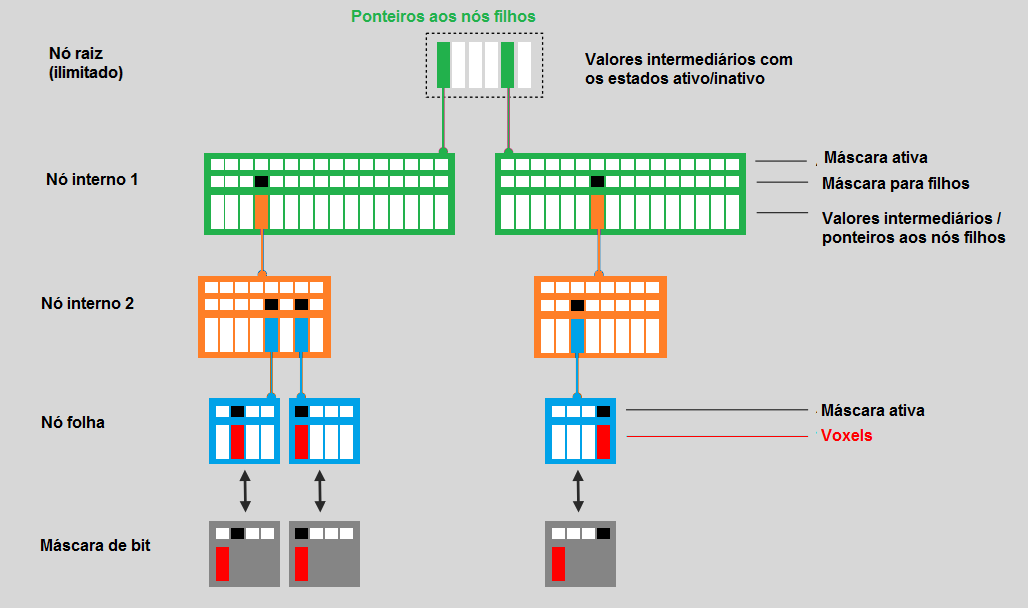
\includegraphics[width=15cm]{tree_inverted}
\caption{Ilustração unidimensional de uma VDB com um nó raiz, dois níveis de nós internos, e folhas. A raiz é dinâmica e esparsa, ao passo que os outros nós são densos e possuem fatores de ramificação que diminuem de cima para baixo, e que são restritos a potências de dois.}
\label{vdbtree}
\end{figure}


\subsection{Algoritmos de Acesso à Estrutura}
São três os tipos de acesso a uma estrutura de dados espacial: aleatório, sequencial e por estêncil. A implementação de cada uma destas formas de acesso será discutida em seguida.

\subsubsection{Acesso aleatório}
O tipo de acesso mais fundamental, e discutivelmente o de mais difícil implementação, é o acesso aleatório a \voxels arbitrários. O que separa este tipo de acesso dos demais é que, no pior caso, cada acesso requer que árvore seja percorrida por inteira, de cima para baixo, começando na raiz e possivelmente terminando numa folha. Na prática, no entanto, o acesso aleatório pode ser melhorado se a ordem de busca na árvore for invertida. Deste modo, é mais fácil definir o acesso aleatório em função dos demais tipos de acesso: acesso aleatório é o tipo de acesso que não é sequencial e não é baseado em estêncis. Estes dois últimos tipos de acesso são facilmente definidos como acesso com um padrão fixo, definido pela organização dos dados na memória ou algum padrão de estêncil. \\

Como a VDB é balanceada em altura por construção com uma profundidade imutável durante a execução, todo caminho entre a raiz \texttt{RootNode} até qualquer uma das folhas \texttt{LeafNode} é igualmente longo e podemos concluir que toda consulta aleatória leva o mesmo tempo no pior caso. Acesso aleatório a valores intermediários armazenados em níveis mais rasos da árvore é mais rápido, já que a busca se encerra antes. \\

\emph{Inserção aleatória} é normalmente usada quando os \grids estão sendo inicializados, mas pode ser importante também para dados dinâmicos e simulações. A busca na árvore é feita como discutido anteriormente, mas agora um nó é alocado se o \bit correspondente não estiver setado em alguma \texttt{mChildMask}. A busca termina em uma folha, possivelmente recém-construída, com o valor do \voxel atribuído no \buffer apropriado e o \bit correspondente setado em \texttt{mValueMask}. Como os nós abaixo da raiz \texttt{RootNode} são alocados apenas na inserção, o consumo de memória para dados volumétricos esparsos é baixo. E embora esta alocação dinâmica de nós implique que a inserção aleatória seja mais lenta que a consulta aleatória, o {\it overhead} é tipicamente amortizado após várias operações de inserção com coerência espacial. \\

\emph{Remoção aleatória} é outro exemplo de uma operação que requer eficiência quando lidamos com dados dinâmicos. A busca é implementada de maneira semelhante à inserção, mas agora os \bits na \texttt{mChildMask} e na \texttt{mValueMask} são desmarcados e os nós são removidos se não possuírem outros filhos ou outros nós ativos. \\

Finalmente, concluímos que a VDB suporta operações aleatórias como consulta, inserção e remoção em tempo constante e isso é, na média, independente da topologia ou resolução do conjunto de dados que estão sendo armazenados.
 
\subsubsection{Acesso sequencial}
Muitos algoritmos acessam ou modificam todos os \voxels ativos em um \grid, mas não dependem da sequência em que isso acontece. Em particular, isso é verdade para a maioria das simulações dependentes do tempo, como advecção de fluidos. Esta invariância pode ser explorada se um padrão de acesso sequencial puder ser definido que tenha um desempenho superior àquele do acesso aleatório. \emph{Acesso sequencial}, portanto, é como nos referimos à sequência ótima de acesso aos dados, dada pela ordem em que os dados estão fisicamente dispostos na memória. Com os avanços em hierarquias sofisticadas de cache e algoritmos de pré-captura de instruções ({\it prefetching}) em CPUs modernos, torna-se especialmente importante obter e processar os dados na ordem em que estão armazenados na memória. \\

O desafio é implementar o acesso sequencial de modo que ele seja mais rápido que o acesso aleatório rápido discutido na seção anterior. O problema se resume a localizar o próximo valor ativo ou nó-filho, e a solução é bastante simples: percorrer as máscaras compactas de acesso direto \texttt{mChildMask} e \texttt{mValueMask} em cada nó. Como são estruturas compactas, são facilmente salvos em cache, e várias entradas (\bits) podem ser processados simultaneamente. Como as máscaras de \bit estão em todos os nós de uma árvore VDB, podemos combinar iteradores em vários níveis da árvore, permitindo a criação de iteradores que percorrem valores de \voxels, valores internos ativos, folhas, entre outras possibilidades.

\subsubsection{Acesso por Estêncil}
Acesso eficiente por estêncil em \grids uniformes é um requisito fundamental para cálculos de diferença finita. Esses métodos aproximam operadores diferenciais com diferenças discretas de valores em um \grid numa vizinhaça local denominada estêncil de suporte. Outras aplicações deste tipo de acesso são interpolação e aplicação de filtros com {\it kernels} de convolução de suporte local. Os tamanhos e formas destes estêncis pode variar bastante dependendo da técnica aplicada. Normalmente, estes métodos de acesso são combinados com acesso sequencial, originando os iteradores de estêncil, um conceito essencial para muitas simulações numéricas.

\section{Comparação da VDB com Estruturas Semelhantes}

\subsection{Octrees}
\label{octrees}

Uma \emph{octree} é uma estrutura de dados em árvore em que cada nó interno possui exatamente 8 nós-filho. O uso mais comum da estrutura é em computação gráfica para particionar o espaço tridimensional subdividindo-o em oito octantes, de forma recursiva, como mostrado na Figura \ref{octree}. \\

No contexto de renderização, modelagem 3D e extração de malhas, esta estrutura é amplamente utilizada. E como citado na seção \ref{vdb_data}, a VDB mantém blocos organizados dinamicamente numa estrutura hierárquica, de modo que estes blocos são folhas da estrutura de árvore e que ficam todas no mesmo nível de profundidade de um grafo acíclico e conectado, com fatores de ramificação grandes, além de variáveis em momento de compilação. Logo, a VDB é balanceada em altura por construção. Octrees, por outro lado, normalmente são árvores altas, com um fator de ramificação limitado a $2$ em cada eixo ($2^3 = 8$). 
Uma característica da octree adotada pela VDB é a capacidade de armazenar valores em nós que não são folhas, funcionando como um \grid multi-nível adaptativo. 

Contudo, uma limitação da VDB é que, apesar de ser uma estrutura de dados hierárquica, ela provavelmente não é a melhor escolha para métodos de amostragem multi-resolução devido aos elevados fatores de ramificação entre os níveis da árvore, e este é um dos motivos que a VDB não substitui octrees quando uma adaptatividade ótima é desejada.

%figura aqui!! :-P
\begin{figure}[!htb]
\center
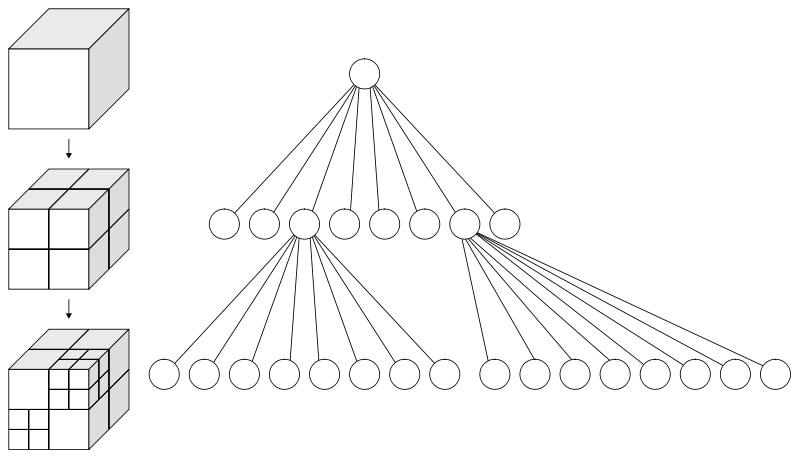
\includegraphics[width=10cm]{Octree2}
\caption{Diagrama de uma octree, estrutura em que cada nó interno possui exatamente oito nós-filho.}
\label{octree}
\end{figure}


\subsection{Árvores B}
Comentaremos brevemente acerca de árvores B para contextualizar a discussão de árvores B+, uma variação da árvore B, na seção \ref{bplus_trees}. \\

Árvore B é uma estrutura de dados que mantém os dados ordenados e permite buscas, acesso sequencial, inserções e remoções em tempo $O(log\;n)$. Trata-se de uma generalização da árvore binária de busca, sendo que esta, a árvore B, pode ter mais de dois filhos por nó. Além disso, esta árvore é otimizada para leitura e escrita de grandes volumes de dados, e por isso tem ampla aplicação em bancos de dados de sistemas de arquivos.

\subsection{Árvores B+}
\label{bplus_trees}
Uma árvore B+ é um árvore n-ária com um número variável, e normalmente grande, de filhos por nó. Uma árvore B+ consiste de raiz, nós internos e folhas. A raiz pode ser uma folha ou um nó com dois ou mais filhos.

Uma árvore B+ é uma árvore B em que cada nó que não seja uma folha possui apenas uma chave, e não pares chave-valor, com um nível a mais nas folhas. A principal aplicação de uma árvore B+ é armazenar dados para consultas rápidas em um contexto orientado a blocos de dados, como sistemas de arquivos.\\

A VDB é basicamente uma variação da árvore B+ com características de Octrees. A VDB preserva as características de desempenho das árvores B+ que resultam do uso de fatores de ramificação variáveis e grandes, mas com otimizações específicas à aplicação volumétrica. Na VDB, os valores armazenados no \grid são indexados por suas coordenadas espaciais em todos os nós da árvore, uma árvore B+ convencional armazena dados genéricos, isto é, de qualquer aplicação, indexados por chaves em um contexto orientado a armazenamento por blocos e somente nas folhas. Em outras palavras, VDB é uma estrutura de dados multi-nível e não usa chaves no sentido tradicional como a árvore B+ o faz. Além disso, em várias implementações as folhas de uma árvore B+ são ligadas umas às outras para permitir uma iteração sequencial rápida, diferentemente da VDB que opta por salvar em cache os caminhos de busca percorridos. Finalmente, nas árvores B+ o custo de uma busca aleatória é logarítmico, ao passo que com a VDB o custo de busca é constante. 
 
%figura aqui!! :-P
\begin{figure}[!htb]
\center
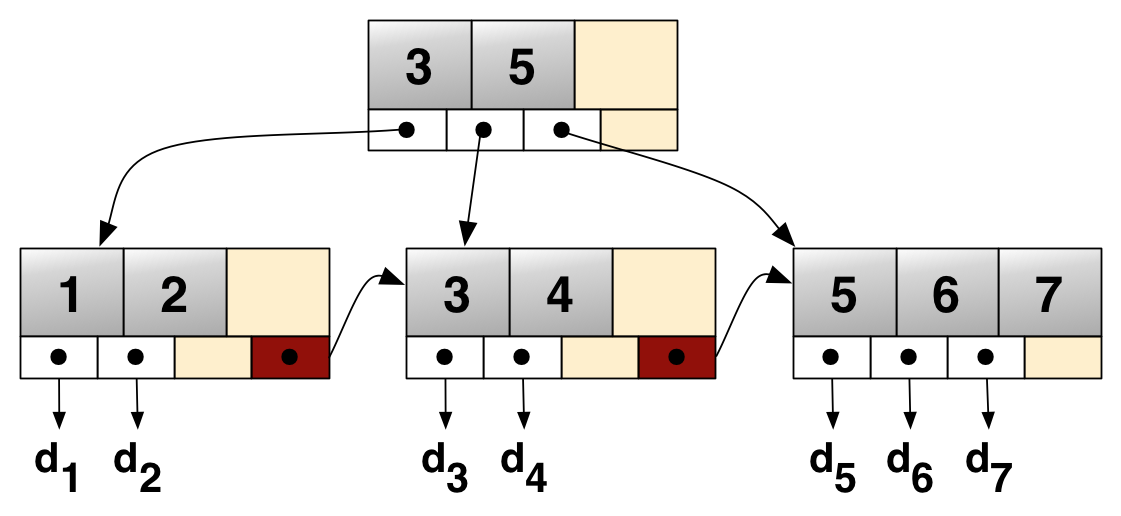
\includegraphics[width=10cm]{Bplustree}
\caption{Diagrama de uma árvore B+. Os números de 1 a 7 são chaves, e os dados armazenados na árvore estão identificados de $d_{1}$ a $d_{7}$.}
\label{bplustree}
\end{figure}



\chapter{Resultados}

%
Para a apresentação dos resultados, é de interesse citar novamente os objetivos estabelecidos no Capítulo \ref{def_problem}. Desejávamos integrar a biblioteca OpenVDB ao Blender, de modo a permitir a visualização de volumes e dados tridimensionais salvos em arquivos desta biblioteca. No entanto, o módulo do software responsável pelos cálculos de iluminação para a exibição do resultado final está em desenvolvimento por outros desenvolvedores e ainda não é funcional.

Por isso, um artifício será utilizado na exibição dos resultados. A consulta aos valores armazenados na textura, ou seja, a amostragem dos pontos será avaliada por fatias, que, neste caso, serão planos, posicionados próximos uns aos outros, de modo a dar a impressão de visualizarmos um volume. A visualização de valores interiores ao volume será dada pelo uso de apenas um plano. Esta estratégia de visualização é exibida na Figura \ref{render_approach}.

%figura aqui!! :-P
\begin{figure}[!htb]
\center
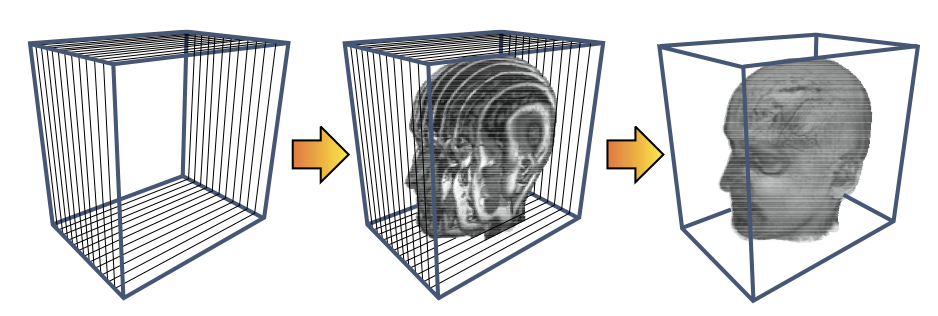
\includegraphics[width=13cm]{2drendering_approach}
\caption{À esquerda, a geometria que conterá os pontos amostrados: uma pilha de planos. No centro, a avaliação dos dados volumétricos em cada uma das fatias. À direita, o resultado da renderização, dando a impressão de visualização de um volume.}
\label{render_approach}
\end{figure}

O volume utilizado para exemplificar o funcionamento da biblioteca no Blender é exibido na Figura \ref{fig:vdb_view1}, e um corte transversal, para visualizarmos seus dados internos, é exibido nas Figuras \ref{fig:vdb_view2} e \ref{fig:vdb_view3}.

\begin{figure}[H]
        \centering
        \begin{subfigure}{0.3\textwidth}
                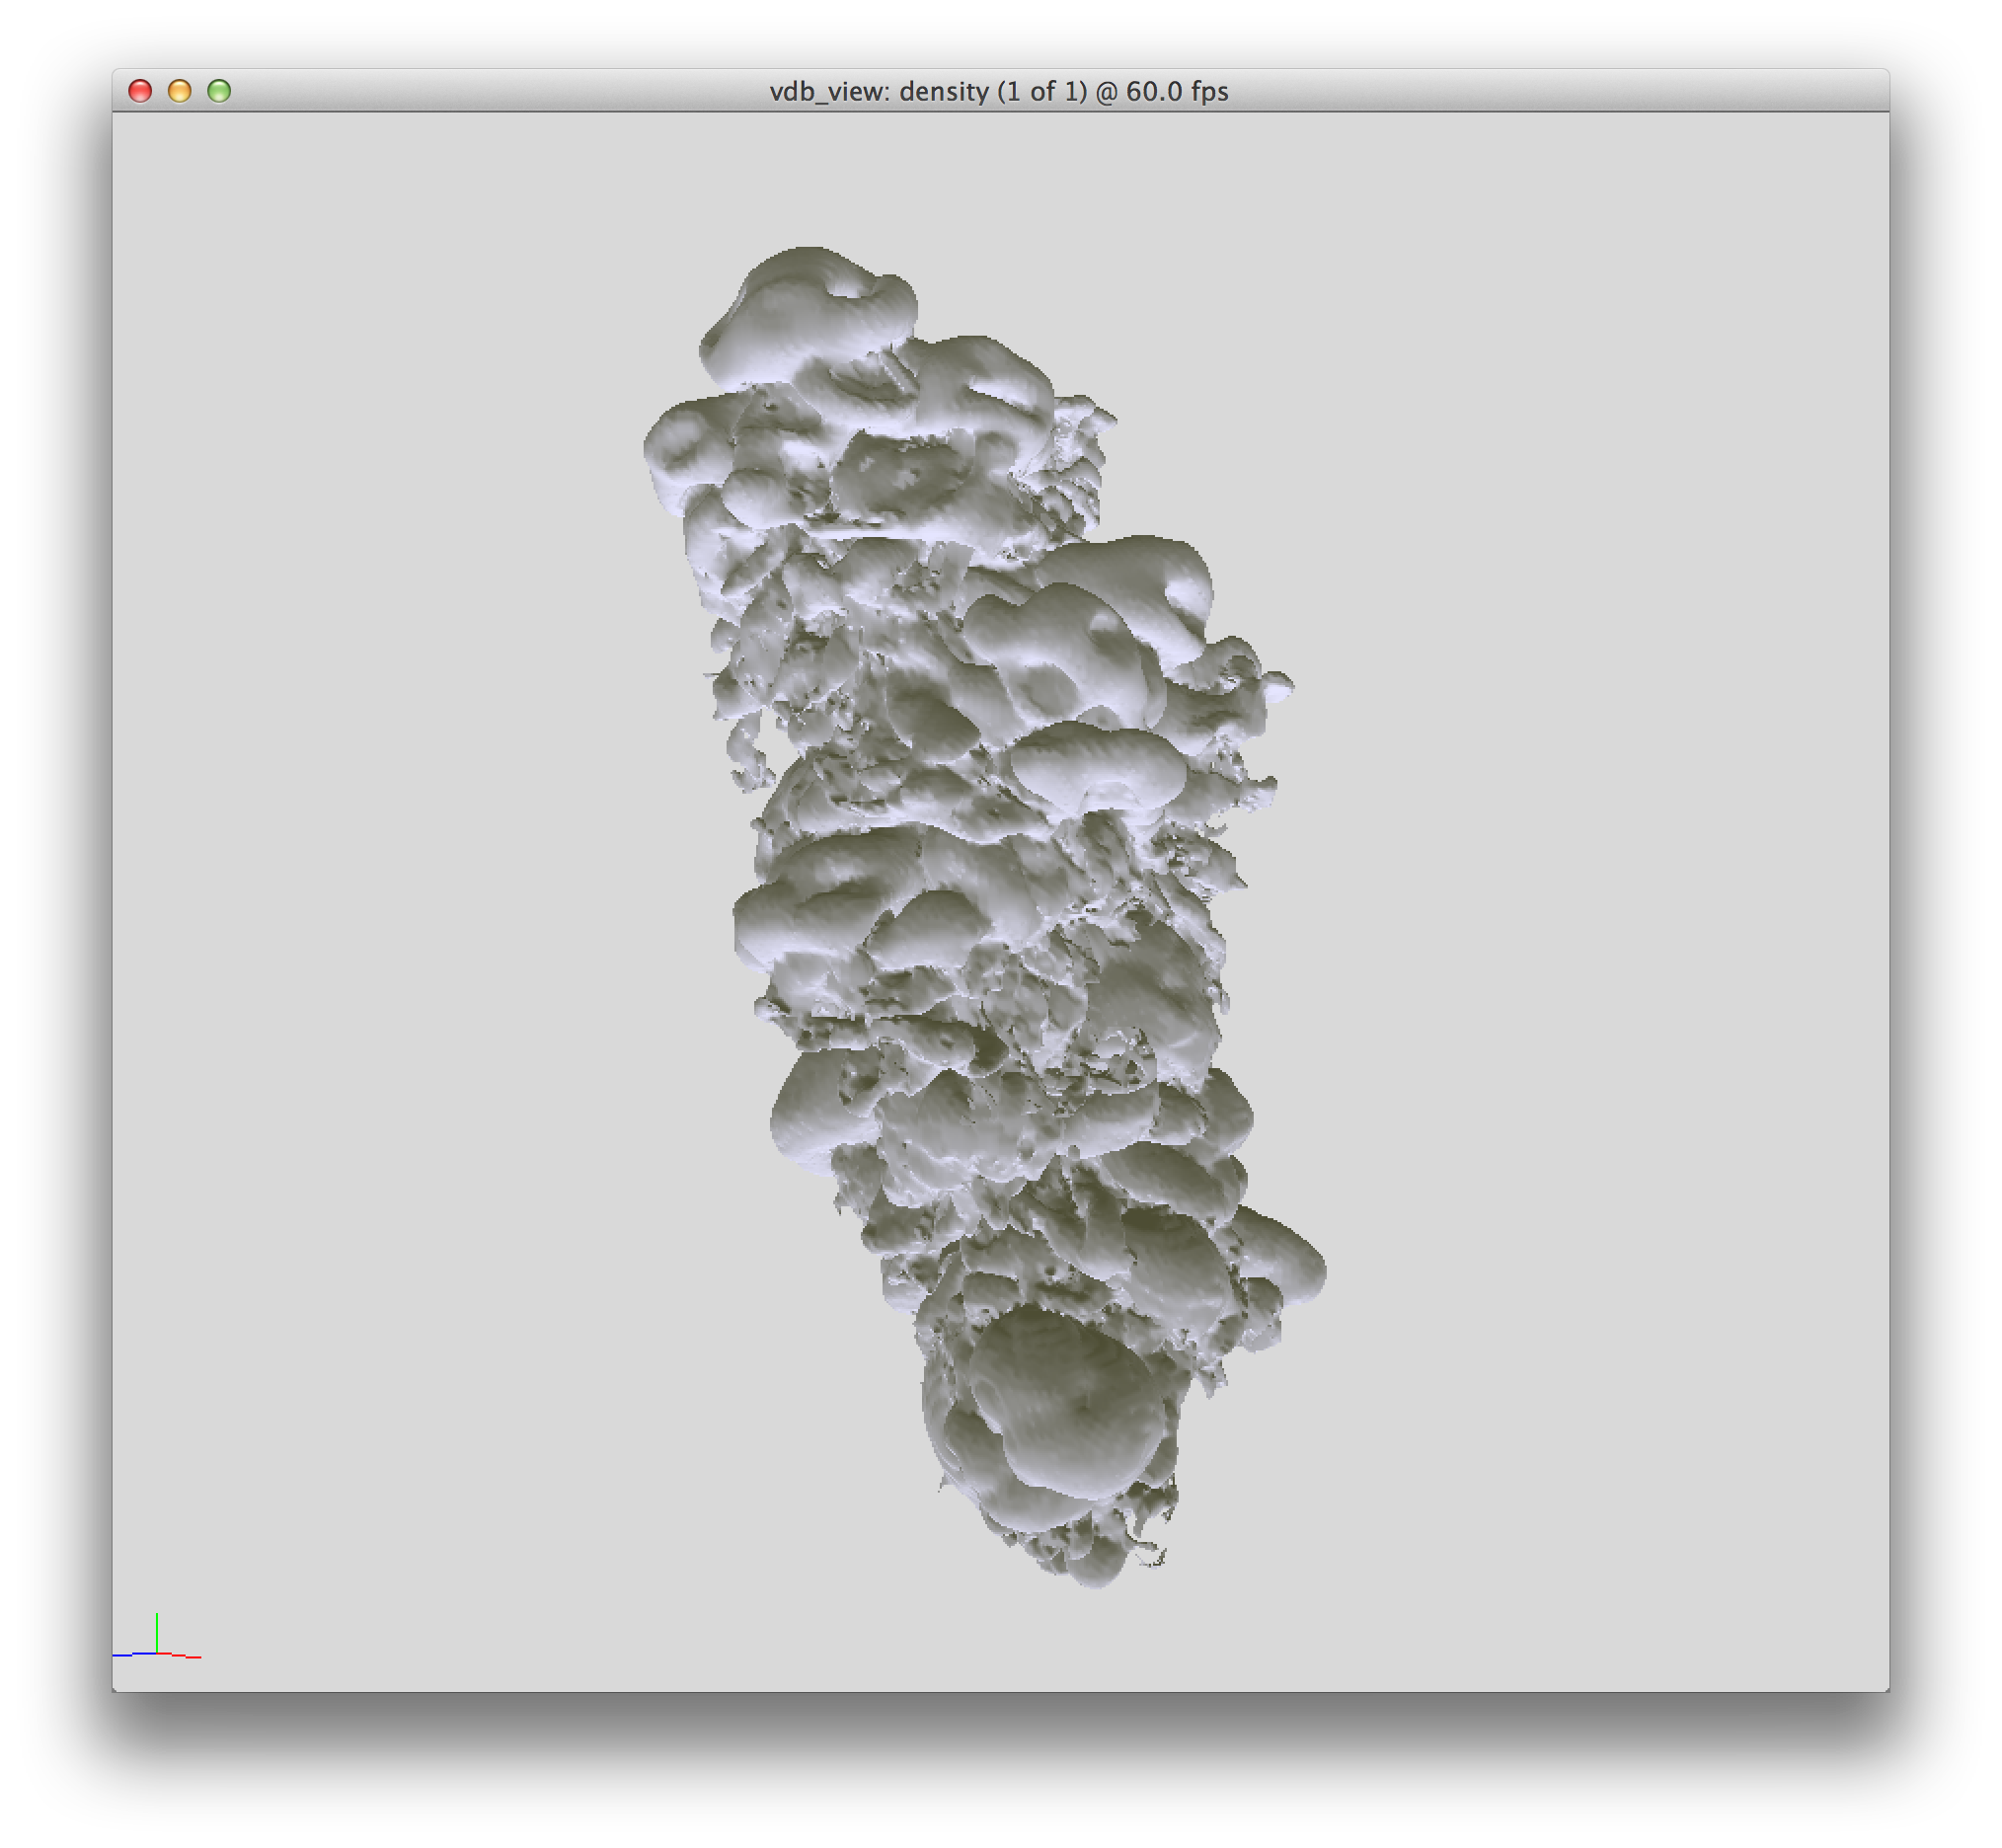
\includegraphics[width=\textwidth]{vdb_view1}
                \caption{Visão externa.}
                \label{fig:vdb_view1}
        \end{subfigure}%
        ~ %add desired spacing between images, e. g. ~, \quad, \qquad etc.
          %(or a blank line to force the subfigure onto a new line)
        \begin{subfigure}{0.3\textwidth}
                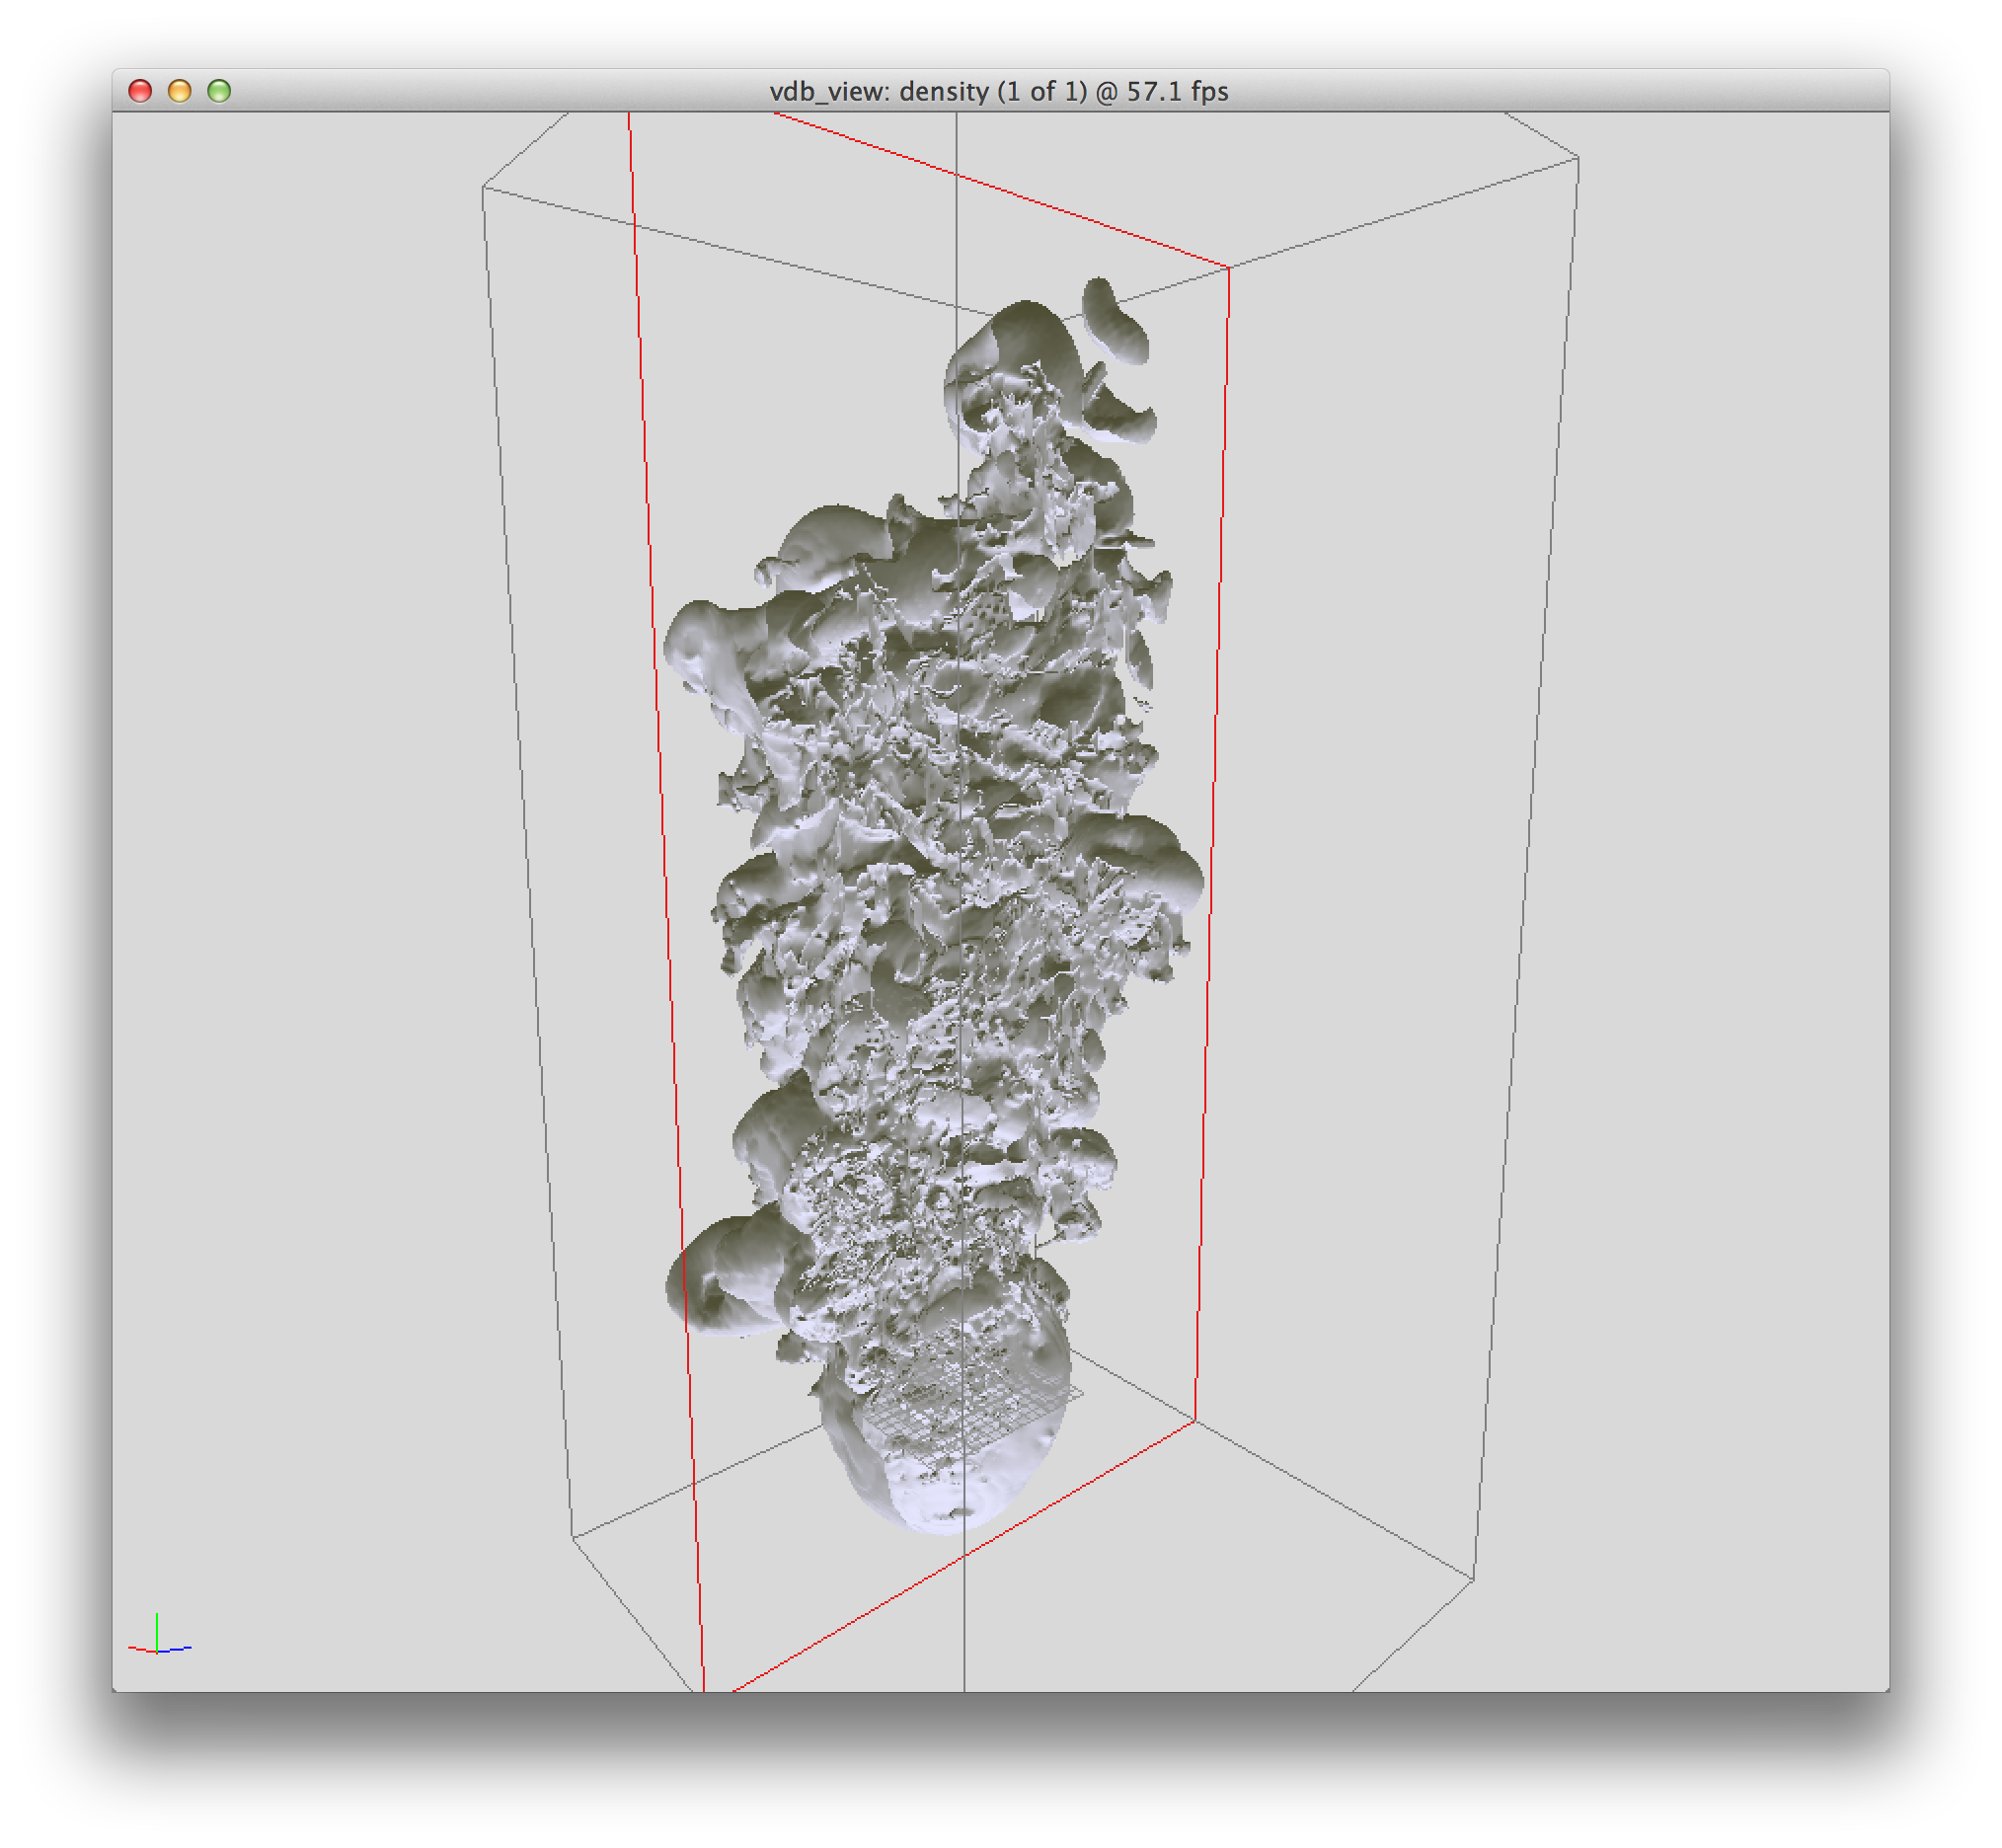
\includegraphics[width=\textwidth]{vdb_view2}
                \caption{Visão interna.}
                \label{fig:vdb_view2}
        \end{subfigure}
        ~ %add desired spacing between images, e. g. ~, \quad, \qquad etc.
          %(or a blank line to force the subfigure onto a new line)
        \begin{subfigure}{0.3\textwidth}
                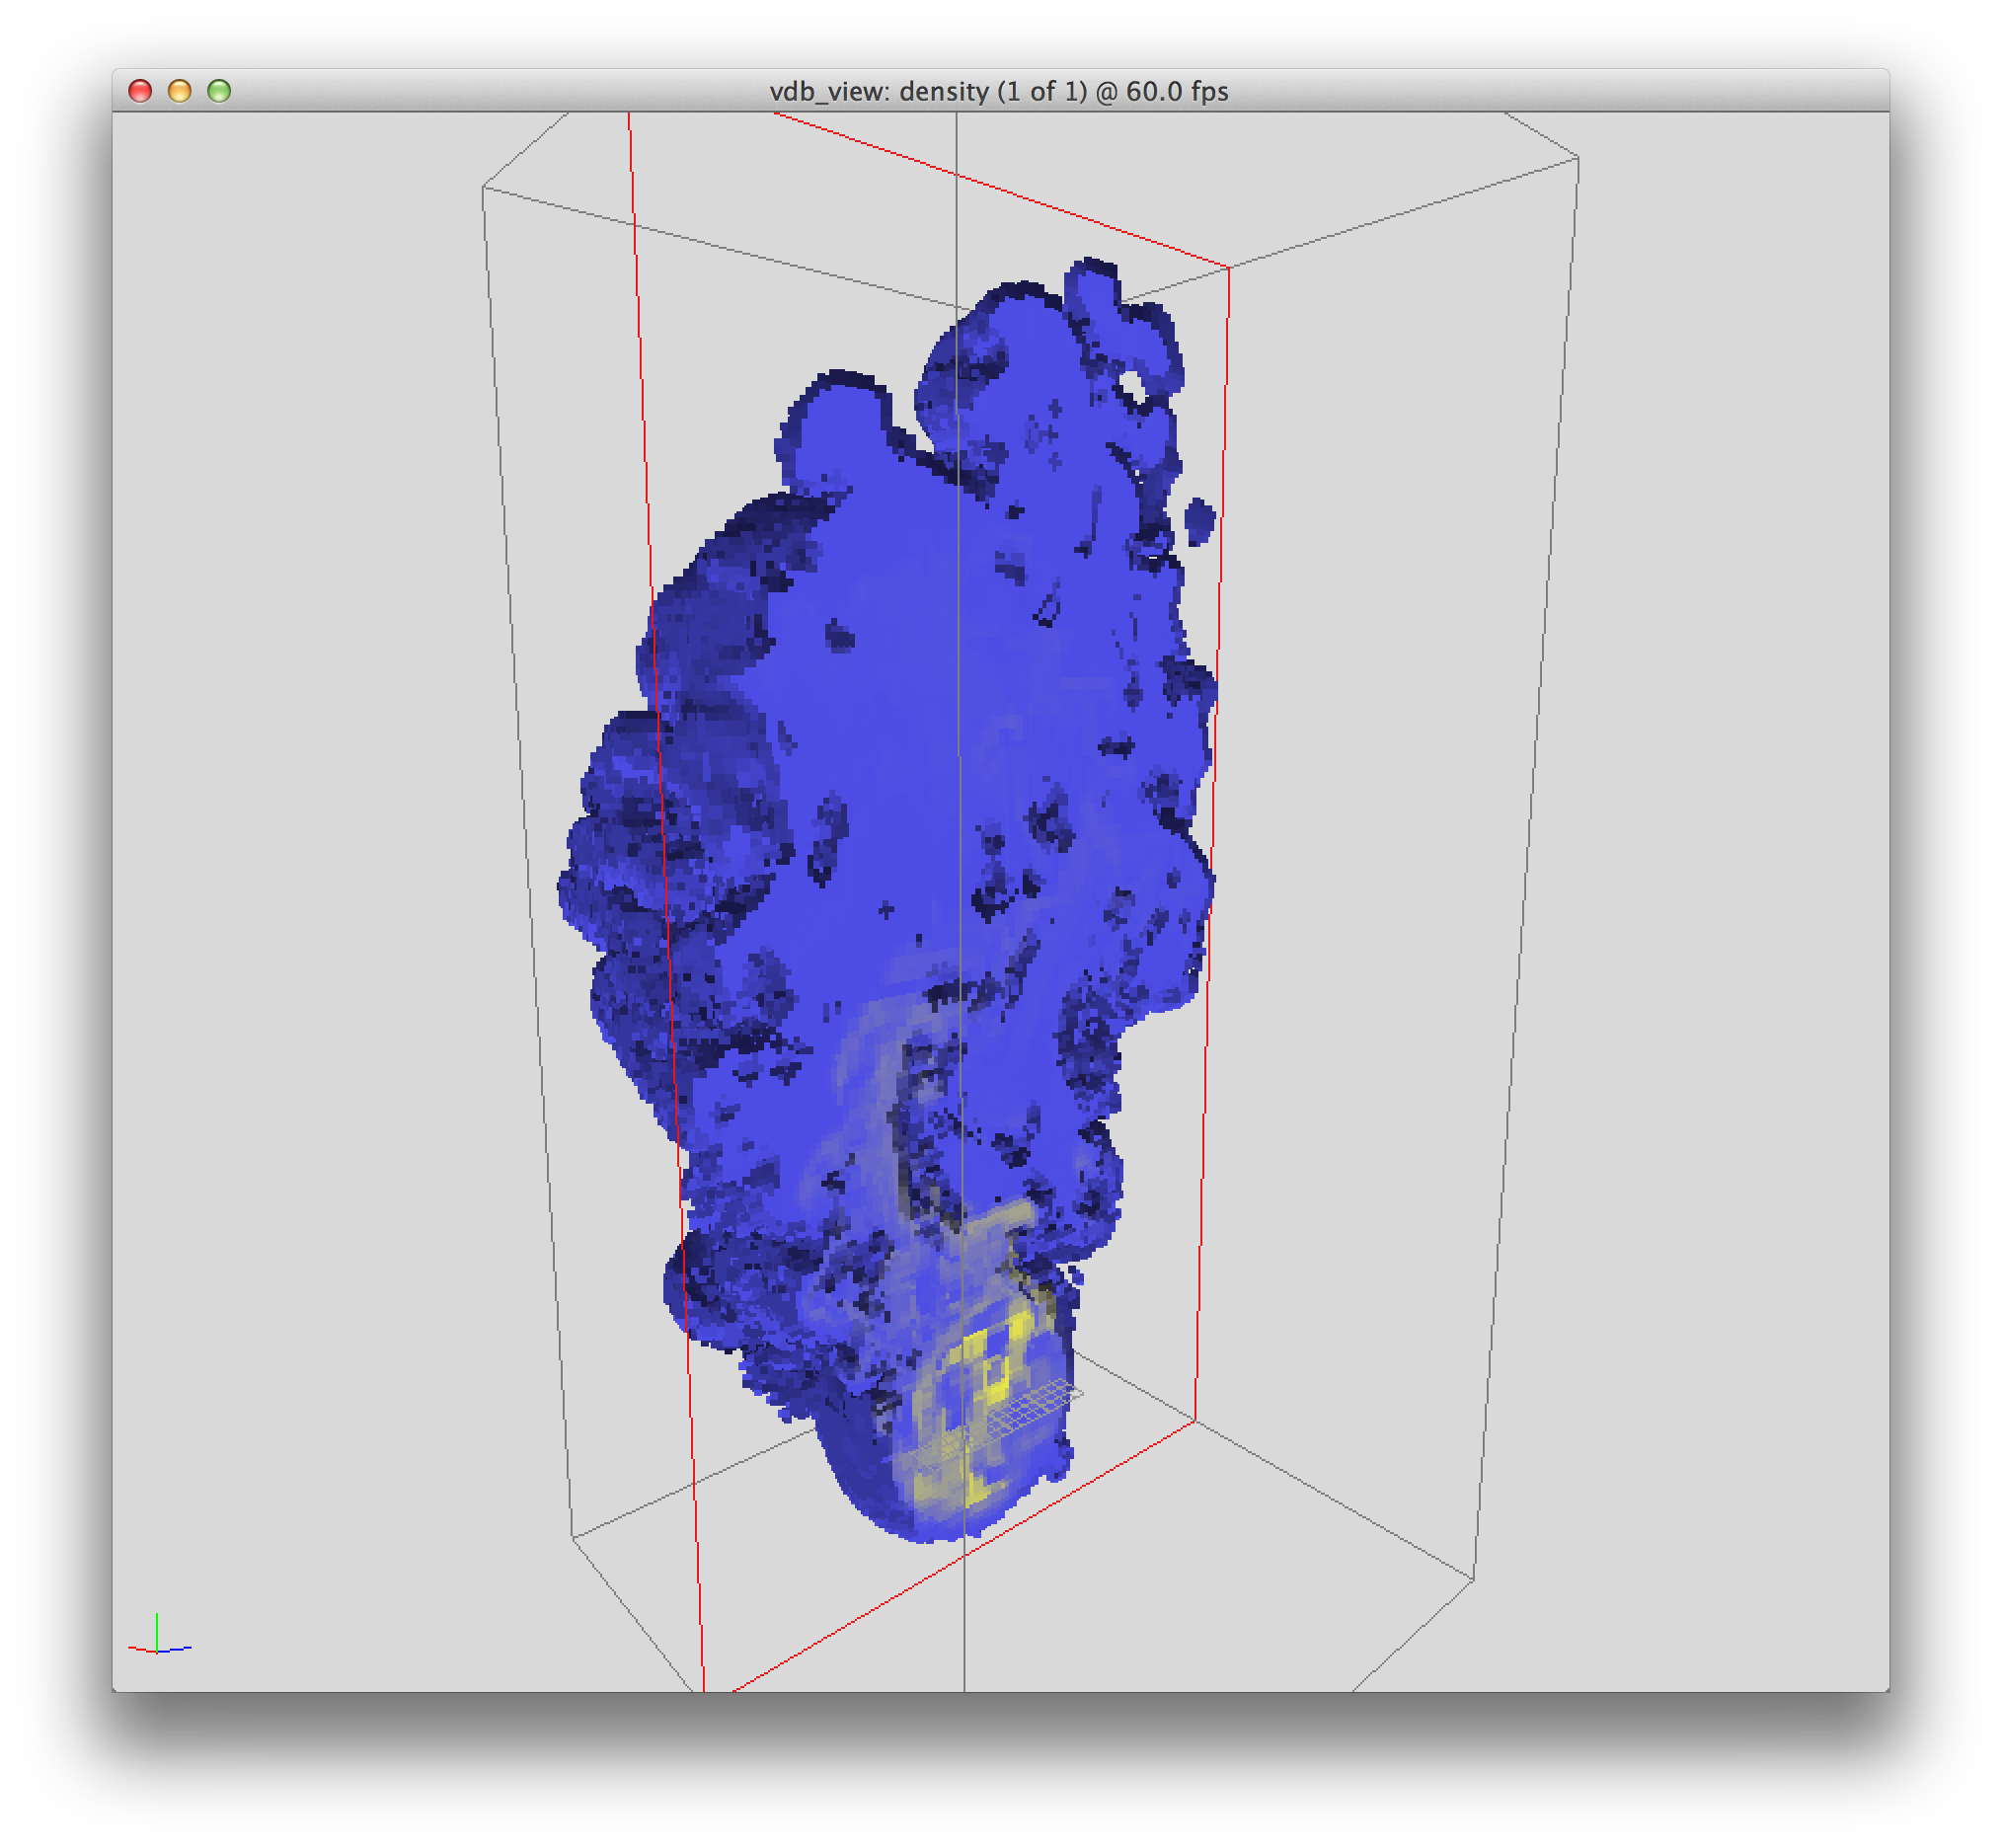
\includegraphics[width=\textwidth]{vdb_view3}
                \caption{Valores, por cor.}
                \label{fig:vdb_view3}
        \end{subfigure}
        \caption{Volume representando a densidade de uma fumaça, usada no exemplo apresentado, exibido por um visualizador específico para o formato VDB.}\label{fig:vdb_view}
\end{figure}


No Blender, o arquivo de exemplo, \texttt{smoke.vdb}, é carregado através de um nó implementado em Open Shading Language, exibido na Figura \ref{vdb_node}. Na Figura \ref{vdb_blender_interface}, a interface do Blender com a pré-visualização do mesmo volume mostrado na Figura \ref{fig:vdb_view} é exibido. As cores de exibição, que estão diferentes entre as representações, são facilmente configuráveis no Blender, se desejado. No Código \ref{log} é mostrada a mensagem escrita em {\it log}, com detalhes do volume carregado. Estes detalhes são obtidos a partir de \emph{metadados} salvos no arquivo e a partir de análise rápida do próprio volume. Na mensagem, a sigla \emph{bbox} refere-se ao \emph{bounding box} do volume, isto é, o menor paralelepípedo alinhado com os eixos do sistema de coordenadas que contém todo o volume. Analogamente, o termo \emph{roi} refere-se à região de interesse, na sigla em inglês. O número de \voxels e o consumo de memória em {\it bytes} também é apresentado. \\

Na Figura \ref{fig:vdb_trans}, são apresentados exemplos de aplicação de \emph{wrapping}, com operações de espelhamento em relação aos eixos y (Figura \ref{fig:vdb_trans2}) e z (Figura \ref{fig:vdb_trans3}). E finalmente, na Figura \ref{planes}, um pequeno número de planos é posicionado na cena, a uma pequena distância uns dos outros, e a textura 3D é então avaliada em cada fatia. À medida que aumentarmos o número de planos, melhor é a impressão de visualizarmos um volume.

\lstinputlisting[label=log,caption=Mensagem exibida em {\it log} quando um arquivo é carregado com sucesso.]{sourceCode/log.cpp}

%figura aqui!! :-P
\begin{figure}[!htb]
\center
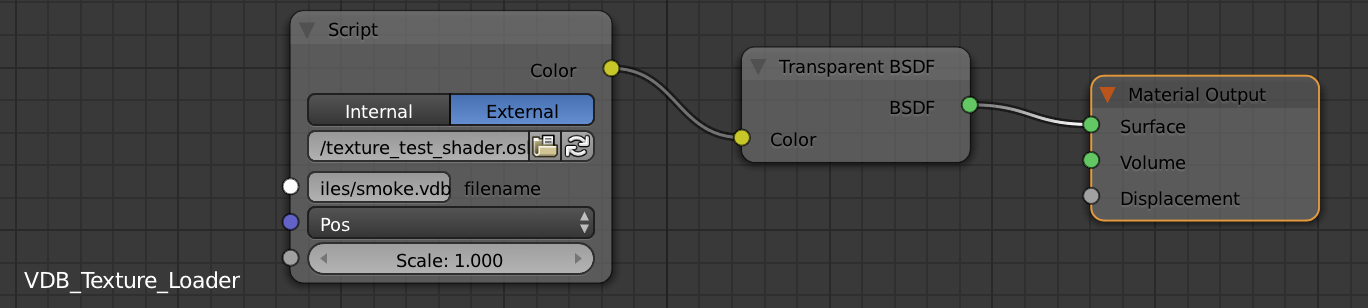
\includegraphics[width=12cm]{vdb_node}
\caption{Nó gerado a partir de código OSL especificamente para carregar arquivos VDB.}
\label{vdb_node}
\end{figure}

%figura aqui!! :-P
\begin{figure}[!htb]
\center
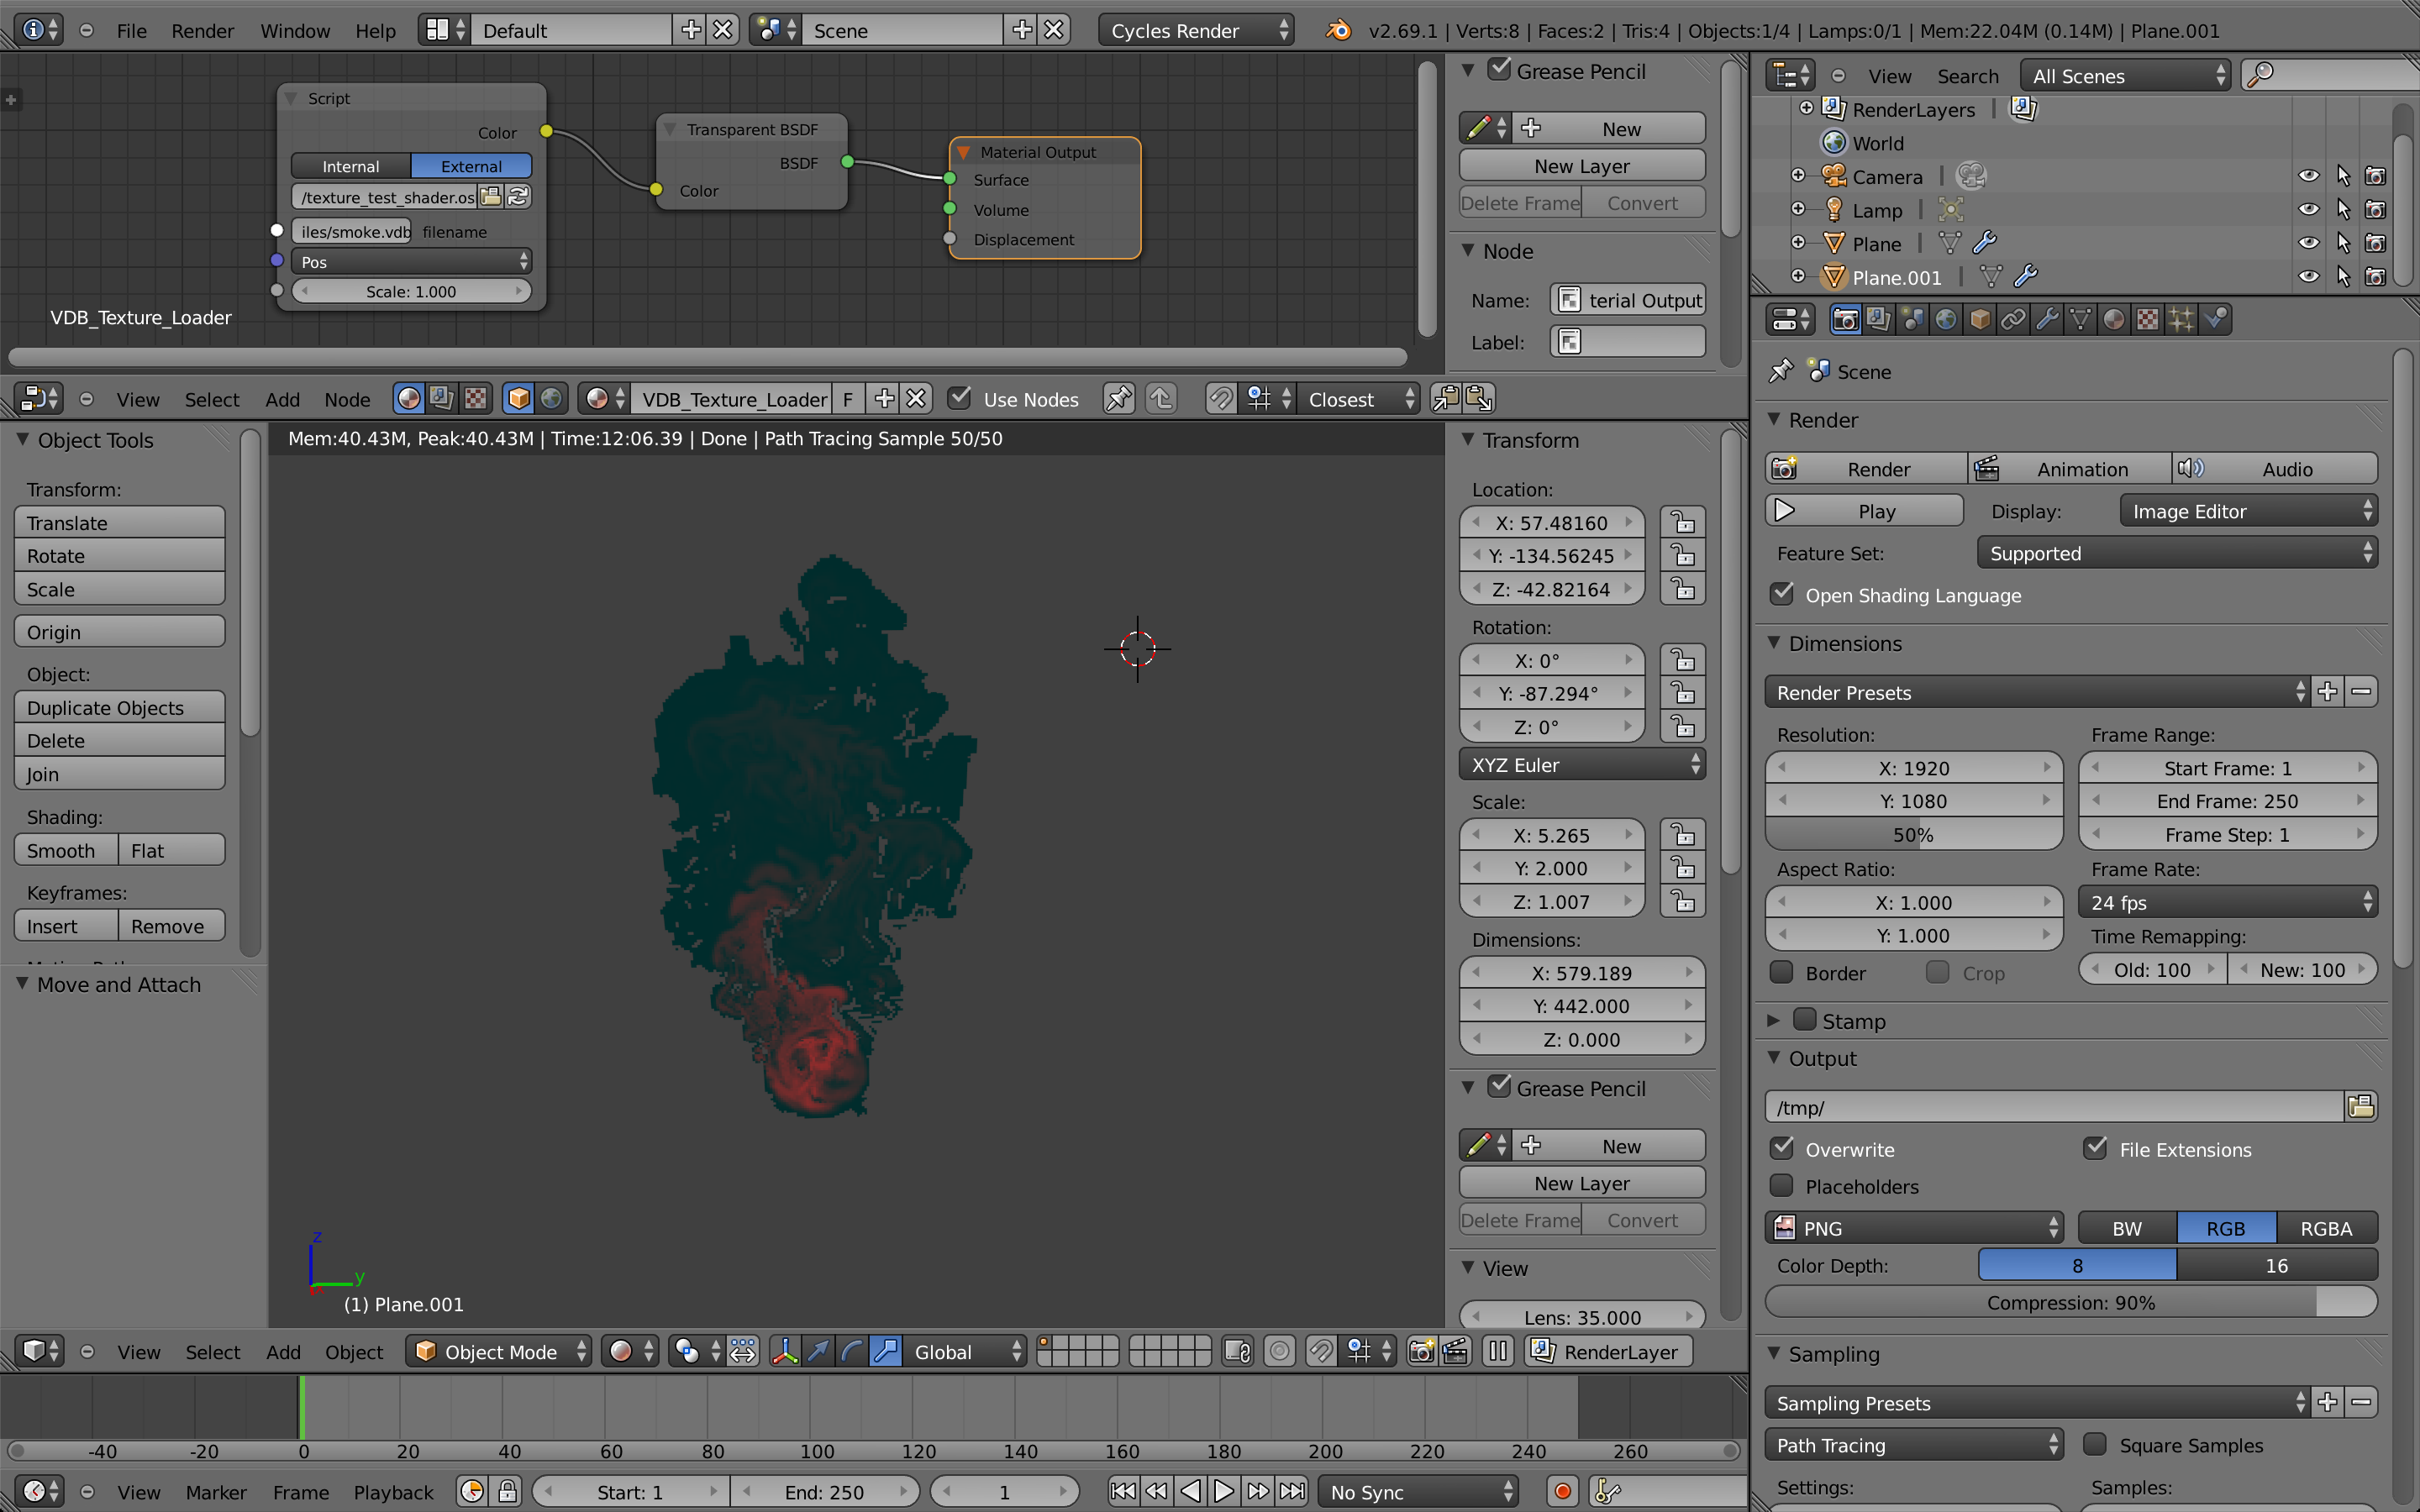
\includegraphics[width=12cm]{vdb_blender_interface}
\caption{Interface do Blender com a pré-visualização de uma fatia do volume.}
\label{vdb_blender_interface}
\end{figure}

\begin{figure}[!htb]
        \centering
        \begin{subfigure}{0.3\textwidth}
                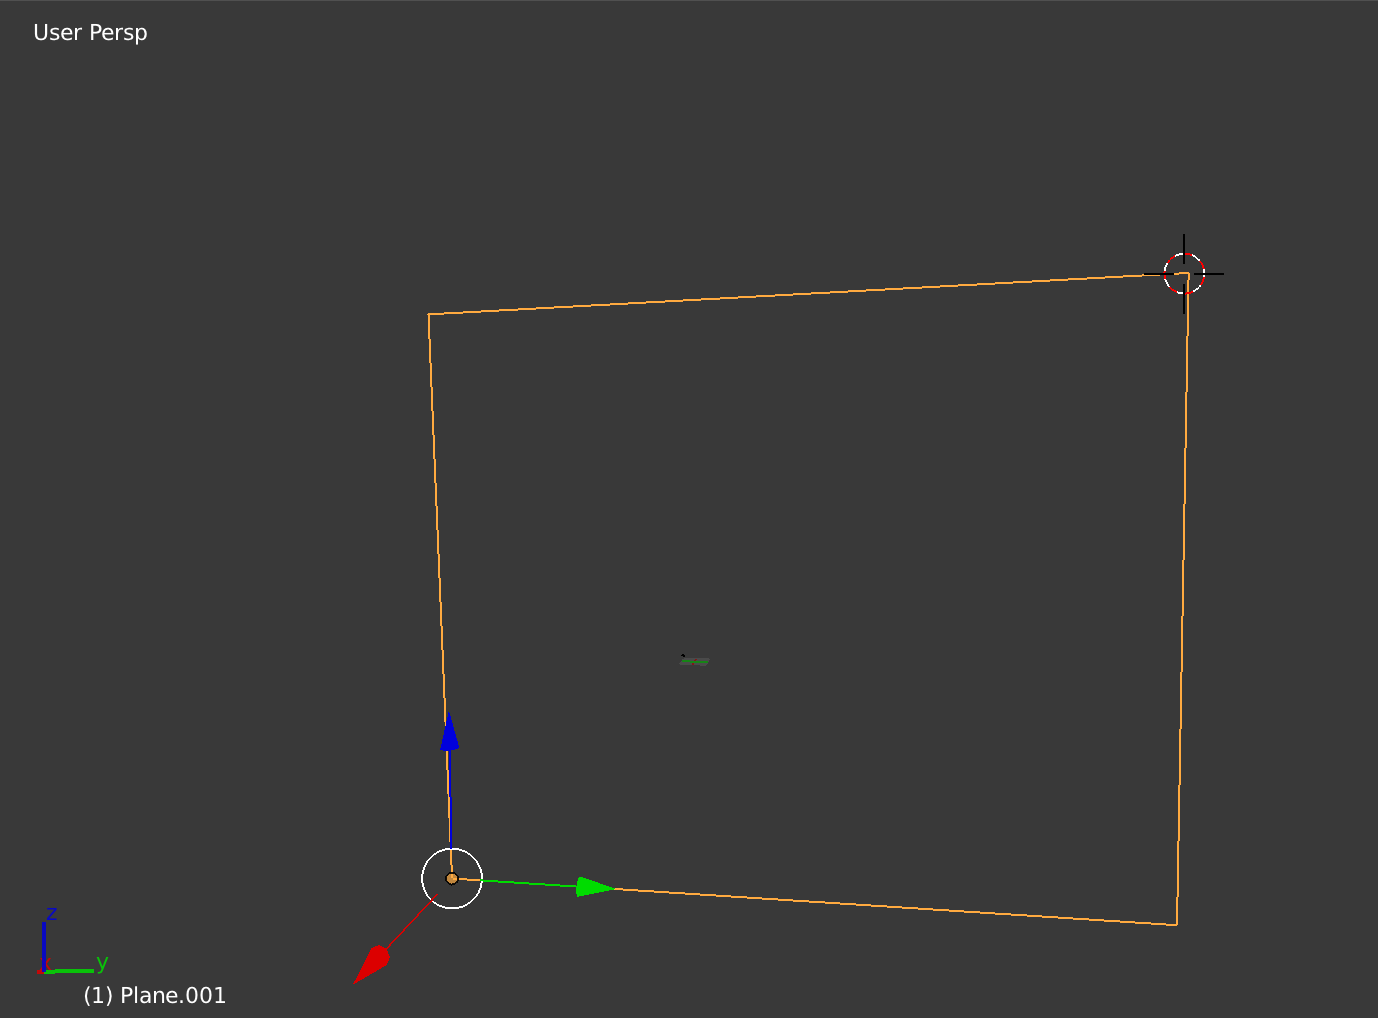
\includegraphics[width=\textwidth]{transf_geometry}
                \caption{Geometria que recebe a textura.}
                \label{fig:vdb_trans1}
        \end{subfigure}%
        ~ %add desired spacing between images, e. g. ~, \quad, \qquad etc.
          %(or a blank line to force the subfigure onto a new line)
        \begin{subfigure}{0.3\textwidth}
                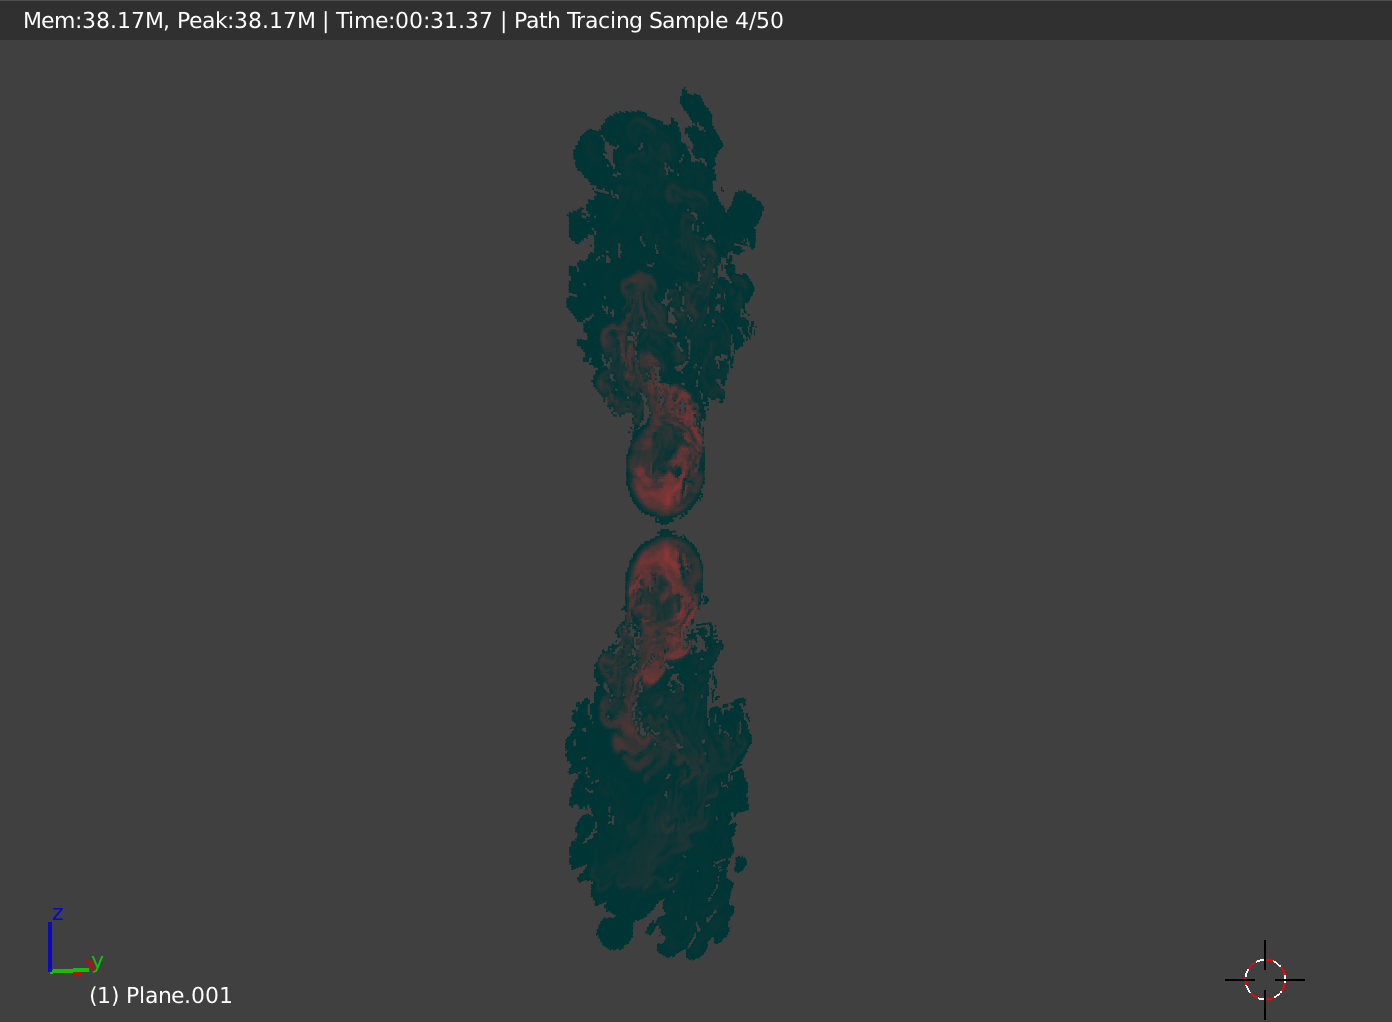
\includegraphics[width=\textwidth]{transf_upsideDown}
                \caption{Espelhamento em torno do eixo Y.}
                \label{fig:vdb_trans2}
        \end{subfigure}
        ~ %add desired spacing between images, e. g. ~, \quad, \qquad etc.
          %(or a blank line to force the subfigure onto a new line
        \begin{subfigure}{0.3\textwidth}
                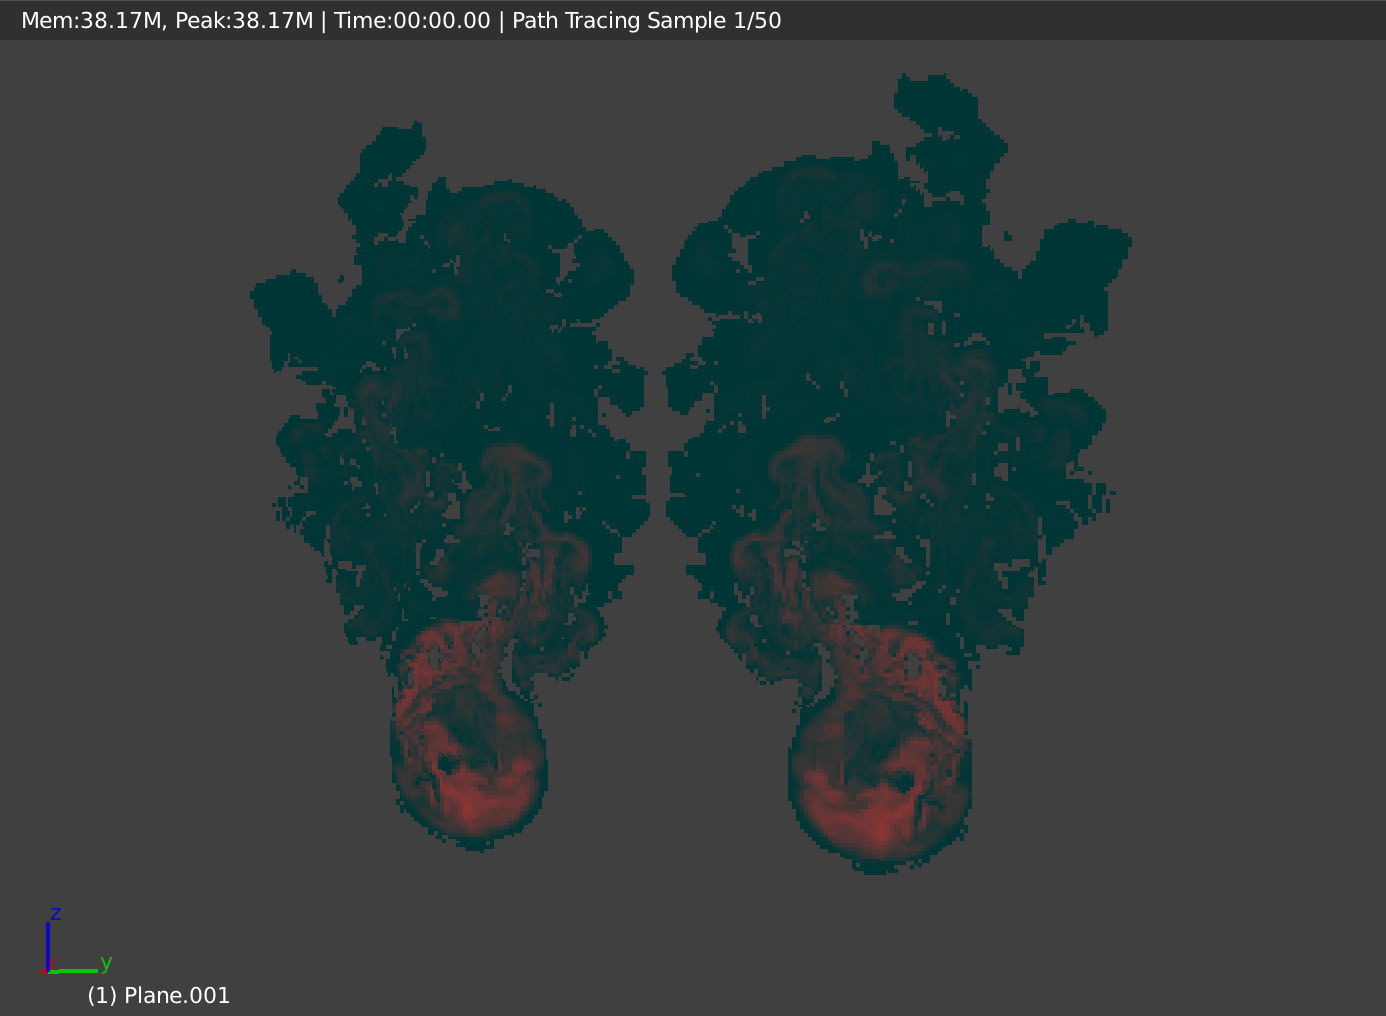
\includegraphics[width=\textwidth]{transf_Mirror}
                \caption{Espelhamento em torno do eixo Z.}
                \label{fig:vdb_trans3}
        \end{subfigure}
        \caption{A mesma fatia de volume exibida na Figura \ref{vdb_blender_interface}, com a aplicação de transformações de espelhamento.}\label{fig:vdb_trans}
\end{figure}


%figura aqui!! :-P
\begin{figure}[!htb]
\center
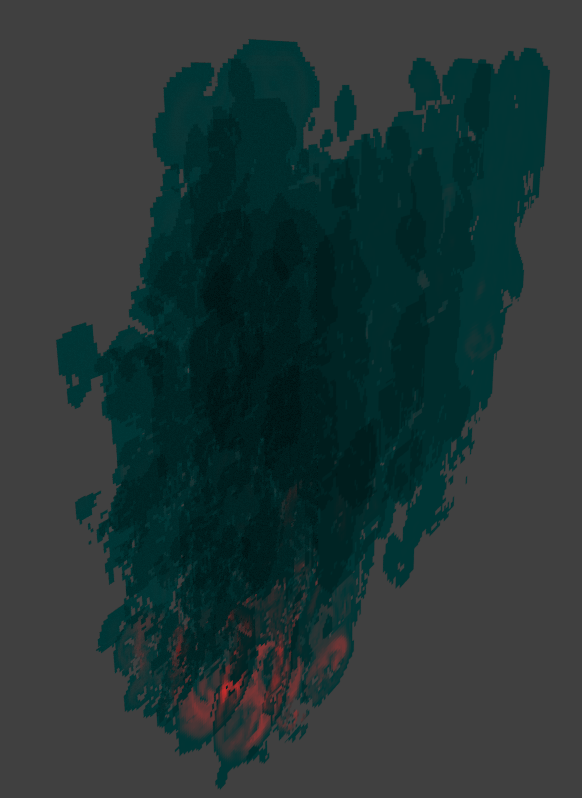
\includegraphics[width=5cm]{multiplePlanes}
\caption{Uma série de planos são posicionados próximos uns aos outros, e o volume é avaliado em cada fatia.}
\label{planes}
\end{figure}

\section*{Análise dos Resultados}

Os resultados encontrados são satisfatórios no sentido de que foi implementado o que foi proposto. Contudo, sua aplicabilidade ainda é limitada, pois depende da implementação do módulo de \emph{shading} para que os volumes em VDB possam ser renderizados de forma apropriada.\\

Ainda assim, a representação de volumes no Blender é agora mais eficiente, e suporta volumes de ordem de grandeza maior que a estrutura anterior, em uma máquina com o mesmo tamanho de memória disponível. Um exemplo é apresentado na Tabela \ref{consumo} para o volume usado neste trabalho, o volume representando uma densidade de fumaça no espaço.

\begin{table}[!ht]
    \centering
        \begin{tabular}{|c|c|c|}
\hline

\multicolumn{3}{|c|}{\bf{Consumo de memória para representação do volume}} \\
\hline \hline
Estrutura de Dados & Consumo de Memória em {\it bytes} & Valor Relativo\\

\hline
 
Vetores 3D (Estrutura existente) & $10.793.640$ &  $1.545$  \\

\hline
 
OpenVDB & $6.984.656$ & $1$ \\

\hline
 

%\hline
\end{tabular}
    \caption{Comparação entre o uso de memória da implementação anterior com o uso da estrutura VDB.}
    \label{consumo}
\end{table}



\chapter{Conclusão}

%
Neste capítulo, os desafios encontrados ao longo do planejamento e implementação deste trabalho serão mencionados, com uma breve explanação. Os resultados obtidos até este momento serão avaliados, e dada a relativa curta duração do projeto para um único desenvolvedor, as funcionalidades que são de interesse e que não foram implementadas ainda serão discutidas no contexto de trabalhos futuros. Finalmente, alguns comentários pessoais acerca do curso de graduação são oferecidos na última seção deste trabalho.

\section{Desafios}

\subsection*{Compilação de código-fonte}

Trabalhar com software multi-plataforma de código aberto oferece alguns desafios inerentes à natureza da metodologia de desenvolvimento necessária. Primeiramente, o código-fonte precisa ser disponibilizado a todos que tiverem interesse em acessá-lo, e isso é essencialmente um problema fechado com os sistemas de versionamento mais modernos, como o \texttt{git}\footnote{http://git-scm.com}. Mas o processo deixa de ser trivial a partir deste ponto: compilar o software, qualquer que seja ele, a partir do código fonte, exige esforço considerável, por vários motivos: obter todas as dependências que o software usa é uma exigência, mas garantir que as versões necessárias são as mesmas que o desenvolvedor instalou é, por si só, um grande desafio, com fatores complicadores como a necessidade de manter múltiplas versões de uma biblioteca para satisfazer pacotes de softwares diferentes, sem que haja interferência entre elas. Neste mesmo cenário, existe ainda a distinção entre o uso de bibliotecas compiladas estática ou dinamicamente, afetando o processo de {\it linking} com mensagens de erro de difícil compreensão. Além disso, variáveis como versão de sistema operacional, de compilador e até mesmo de dispositivos de hardware, como versão de OpenGL suportada pela placa gráfica do desenvolvedor afetam o processo de compilação a partir do código-fonte.\\

Neste trabalho, compilar a biblioteca OpenVDB para uso com o Blender apresentou vários destes desafios, e a solução encontrada foi compilar a biblioteca como parte da solução do Blender, de modo que compartilhassem todas as características de compilação, já que existem dependências em comum, e como resultado, diferenças nas variáveis de compilação deixaram de existir. 


\subsection*{Identificação de Vazamentos de Memória}
O uso de ponteiros em C e C++ não é exatamente trivial. E quando lida-se com arquivos em disco, o custo das operações de E/S normalmente são os fatores de maior impacto no desempenho da aplicação. Logo, ficou claro desde o início que o arquivo em que o volume estava armazenado deveria permanecer aberto, em memória, durante todo o processo de geração de imagens. Para isso, utilizou-se um ponteiro comum para uma estrutura criada que continha o arquivo. De posse do ponteiro, acessava-se o arquivo em memória.\\

A solução adotada funcionava inicialmente para pequenos casos de testes, mas causava o encerramento da aplicação após vários testes seguidos. Casos de teste maiores não eram concluídos. Os ponteiros saíam de escopo após cada sessão de geração de imagem, sem que fossem desalocados de forma apropriada. Após várias execuções, a quantidade de memória perdida era grande demais para manter a aplicação aberta.\\

A solução, sugerida por outros desenvolvedores, foi a adoção de \emph{smart pointers}, ponteiros com alocação dinâmica de memória que garantem que a memória utilizada será desalocada quando o contador de referências ativas atingir zero. Como o funcionamento destes é ligeiramente diferente, a substituição não foi imediata, mas com os devidos ajustes no código, os vazamentos de memória cessaram.

\subsection*{Transformações, Espaços e Sistemas de Coordenadas}
Os arquivos de volume {\it .vdb} definem seus próprios espaços, em que o volume armazenado está contido, e a relação entre seu sistema de coordenadas com aquele da cena utilizada no Blender não é clara. Além disso, as dimensões da imagem volumétrica pode ser ou muito maior ou muito menor que as dimensões da cena que a utilizará. Como consequência, ao importar um volume VDB em uma cena, a visualização nem sempre era possível, ou apenas um fragmento da textura ficava visível. \\

O desafio aqui, na realidade, estava no conceito do problema, pois a diferença entre espaços é natural. A solução foi adotar o objeto em que a textura está sendo avaliada como referência, e mapear, usando uma transformação linear, as coordenadas da textura para as coordenadas do mundo correspondentes. A transformação foi composta usando as coordenadas do objeto, e construindo a matriz $4 \times 4$ para a transformada afim.

\section{Trabalhos Futuros}

Muito embora o trabalho essencial tenha sido executado - agora existe suporte para abrir e visualizar volumes VDB no Blender, não houve tempo hábil para a conclusão de funcionalidades desejáveis, sendo que as principais são listadas a seguir.

\begin{itemize}
\item \emph{Suporte à execução paralela}.
O processo de geração de imagens é de alta complexidade computacional por natureza. E nas operações de avaliação de valores em uma estrutura de dados volumétrica as operações normalmente são altamente paralelizáveis, embora seja necessário tomar alguns cuidados, como preservar a integridade da estrutura na memória. Dessa forma, uma análise é necessária para averiguação de quais operações podem ser paralelizadas sem risco, verificando ainda se modificações na implementação atual podem favorecer a paralelização do código.

\item \emph{Criação de interface de usuário}. A interface usada atualmente entre o Blender e a estrutura de dados é um {\it shader} escrito em \emph{Open Shading Language}. A criação de um nó específico para este fim - importar volumes VDB previamente salvos - facilitaria o processo. Este nó ficaria acessível a partir de um dos menus no software.

\item \emph{Permitir que volumes do Blender sejam exportados em VDB}. O Blender possui um simulador de fumaça bastante sofisticado, e há interesse em salvar estes volumes, que atualmente são gerados e salvos como volumes densos, no formato VDB. Um conversor entre as duas representações precisa ser implementado para este fim.

\end{itemize}

\section{Comentários Finais}

Um dos aspectos mais interessantes de lidar com um problema de mundo real de uma aplicação deste gênero é a realização de que assuntos e disciplinas aparentemente sem relação alguma entre si convergem para permitir a solução de um problema. O uso de métodos de \emph{Cálculo Numérico} para a implementação de técnicas estudadas em \emph{Análise de Sinais e Sistemas}, por exemplo, teria sido uma aplicação de interesse na ocasião em que estes tópicos foram estudados pela primeira vez durante o curso de graduação. \\

Um outro ponto importante é a aplicação direta de conceitos e práticas sugeridas em cursos como o de \emph{Engenharia de Software}, como a configuração de software e as dificuldades em manter um conjunto de alterações em desenvolvimento isoladas da distribuição principal, mas mantendo a sincronização das alterações feitas à distribuição principal para que o software em desenvolvimento não fique obsoleto. \\

E finalmente, as disciplinas de \emph{Álgebra Linear} e \emph{Computação Gráfica} apresentaram os fundamentos para permitir a compreensão do problema, antes mesmo de tentar atacá-lo. \\

Em termos profissionais, a experiência foi bastante favorável pela comunicação com pessoas influentes da área de computação gráfica, e que sempre se mostraram bastante disponíveis para os interessados em aprender e desenvolver software novo. Além disso, depois de sofridas sessões de revisões de código, é muito gratificante ter código de sua autoria em um repositório público.

\iffalse
1. introdução (4)
 1.1 definição do problema / objetivo
 1.2 motivação
 1.3 sobre o projeto pessoal

2. estrutura de dados (10)
 2.1 definição
 2.2 relação com outras estruturas

3. blender (10)
 3.1 textura 
  3.1.1 definição
  3.1.2 mapeamento
  3.1.3 tiles
  3.1.4 3d
 3.2 sistemas de coordenadas
  3.2.1 WCS
  3.2.2 ObjSpace
  3.2.3 coordenadas da textura, mapeamento uv
3.3 shaders / OSL
 3.3.1 interface com estruturas / textura

4. resultados (5)
 4.1 imagens
 4.2 referências à teoria
 4.3 tempo / benchmark

5. conclusão
 5.1 desafios encontrados
 5.2 análise resultados
 5.3 ganhos pessoais / disciplinas / projetos 

\fi



\end{document}